\chapter{Data verses MC in control regions} % Main appendix title

\label{AppendixC}
\section{e/$\mu$ + $\gamma$ control region}
\begin{figure}[h!]
\centering
\caption[Data vs MC for $e\gamma$ CR]{Distribution of $e+\gamma$ events versus \ptmiss (top left), \ST (top right), 
\mt (middle left), $p_{T,e}$ (middle right), \nj (bottom left), \nb (bottom right).  
Filled histograms denoted expected yields from MC for various processes.  Markers represent data yields.
MC event yields are scaled to the same integrated luminosity as data.}
\label{fig:lost_e_CR_dist}
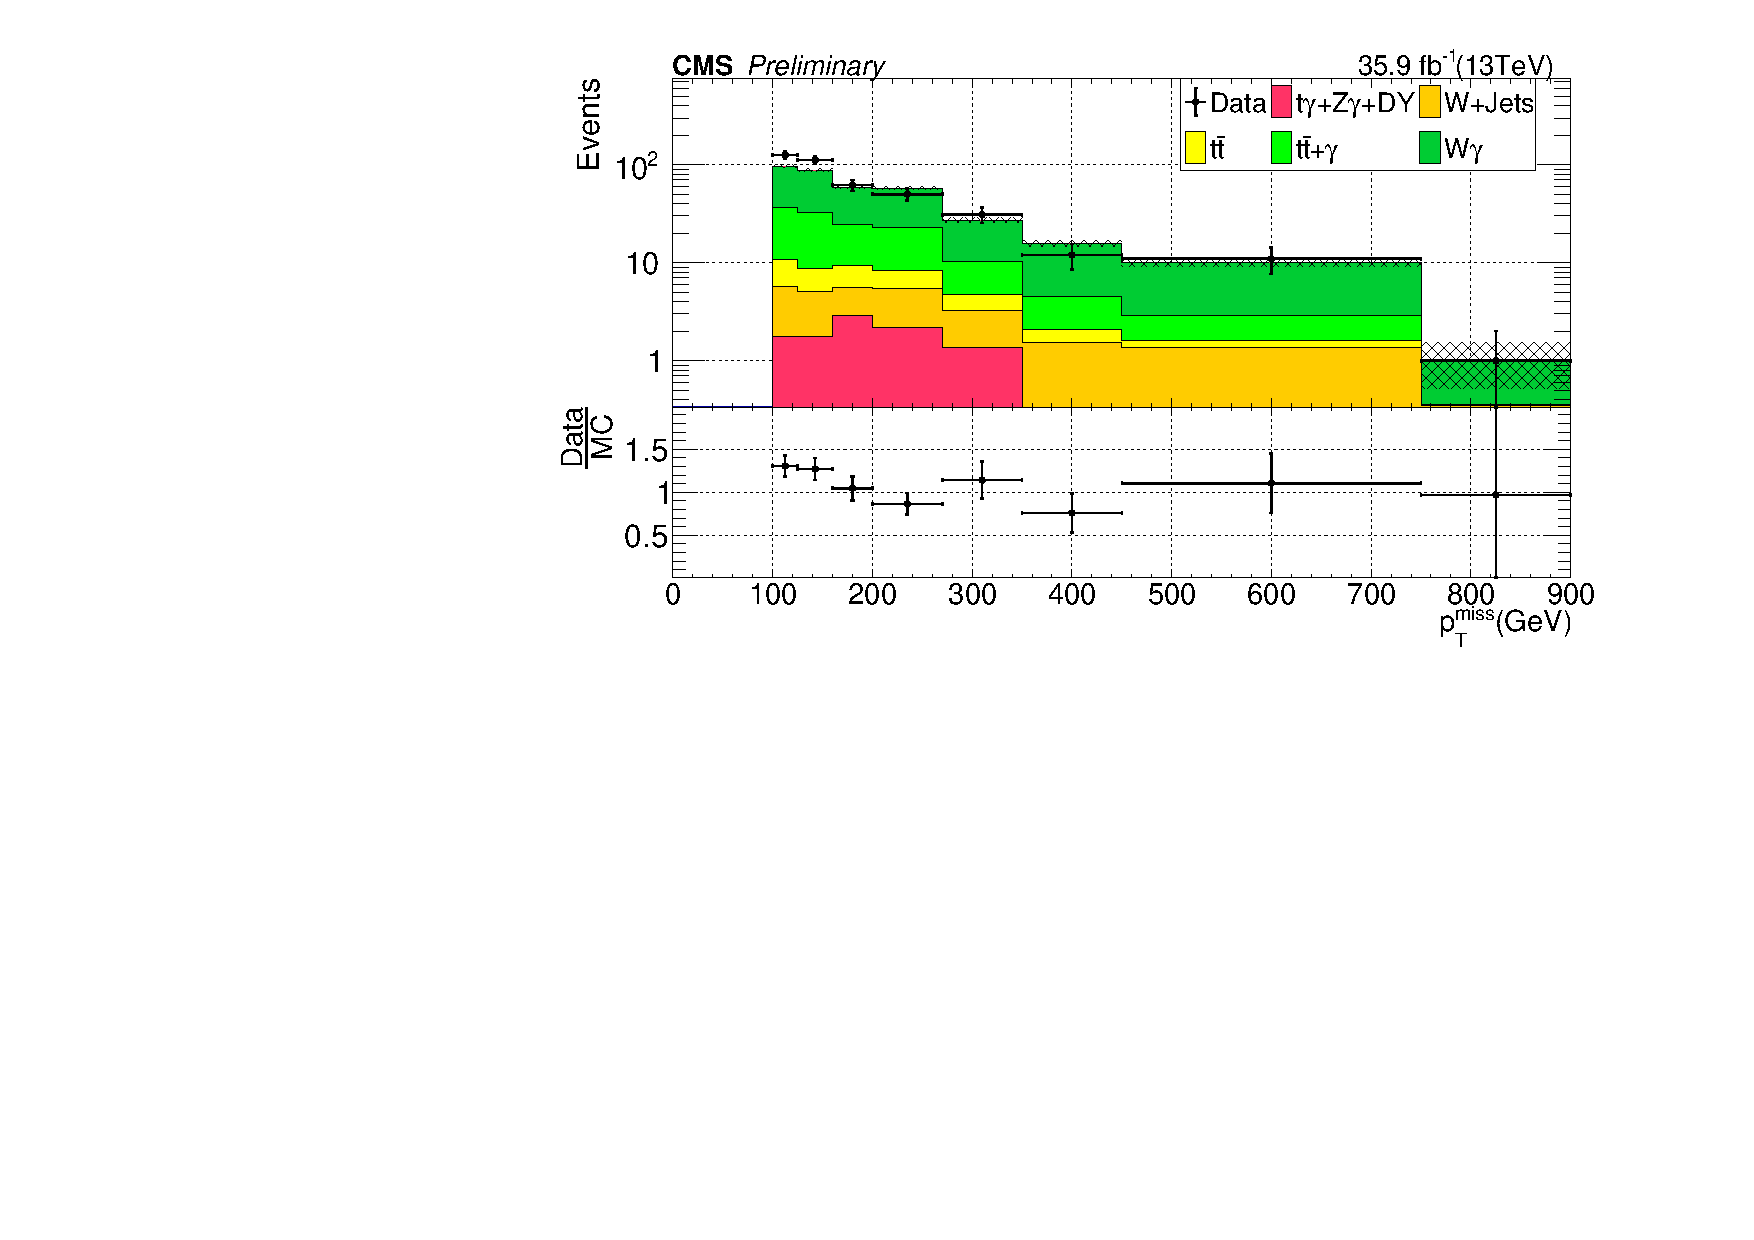
\includegraphics[width=0.48\linewidth]{../Figures/Chap3/lost_lepton/METvarBin_Ele1.pdf}
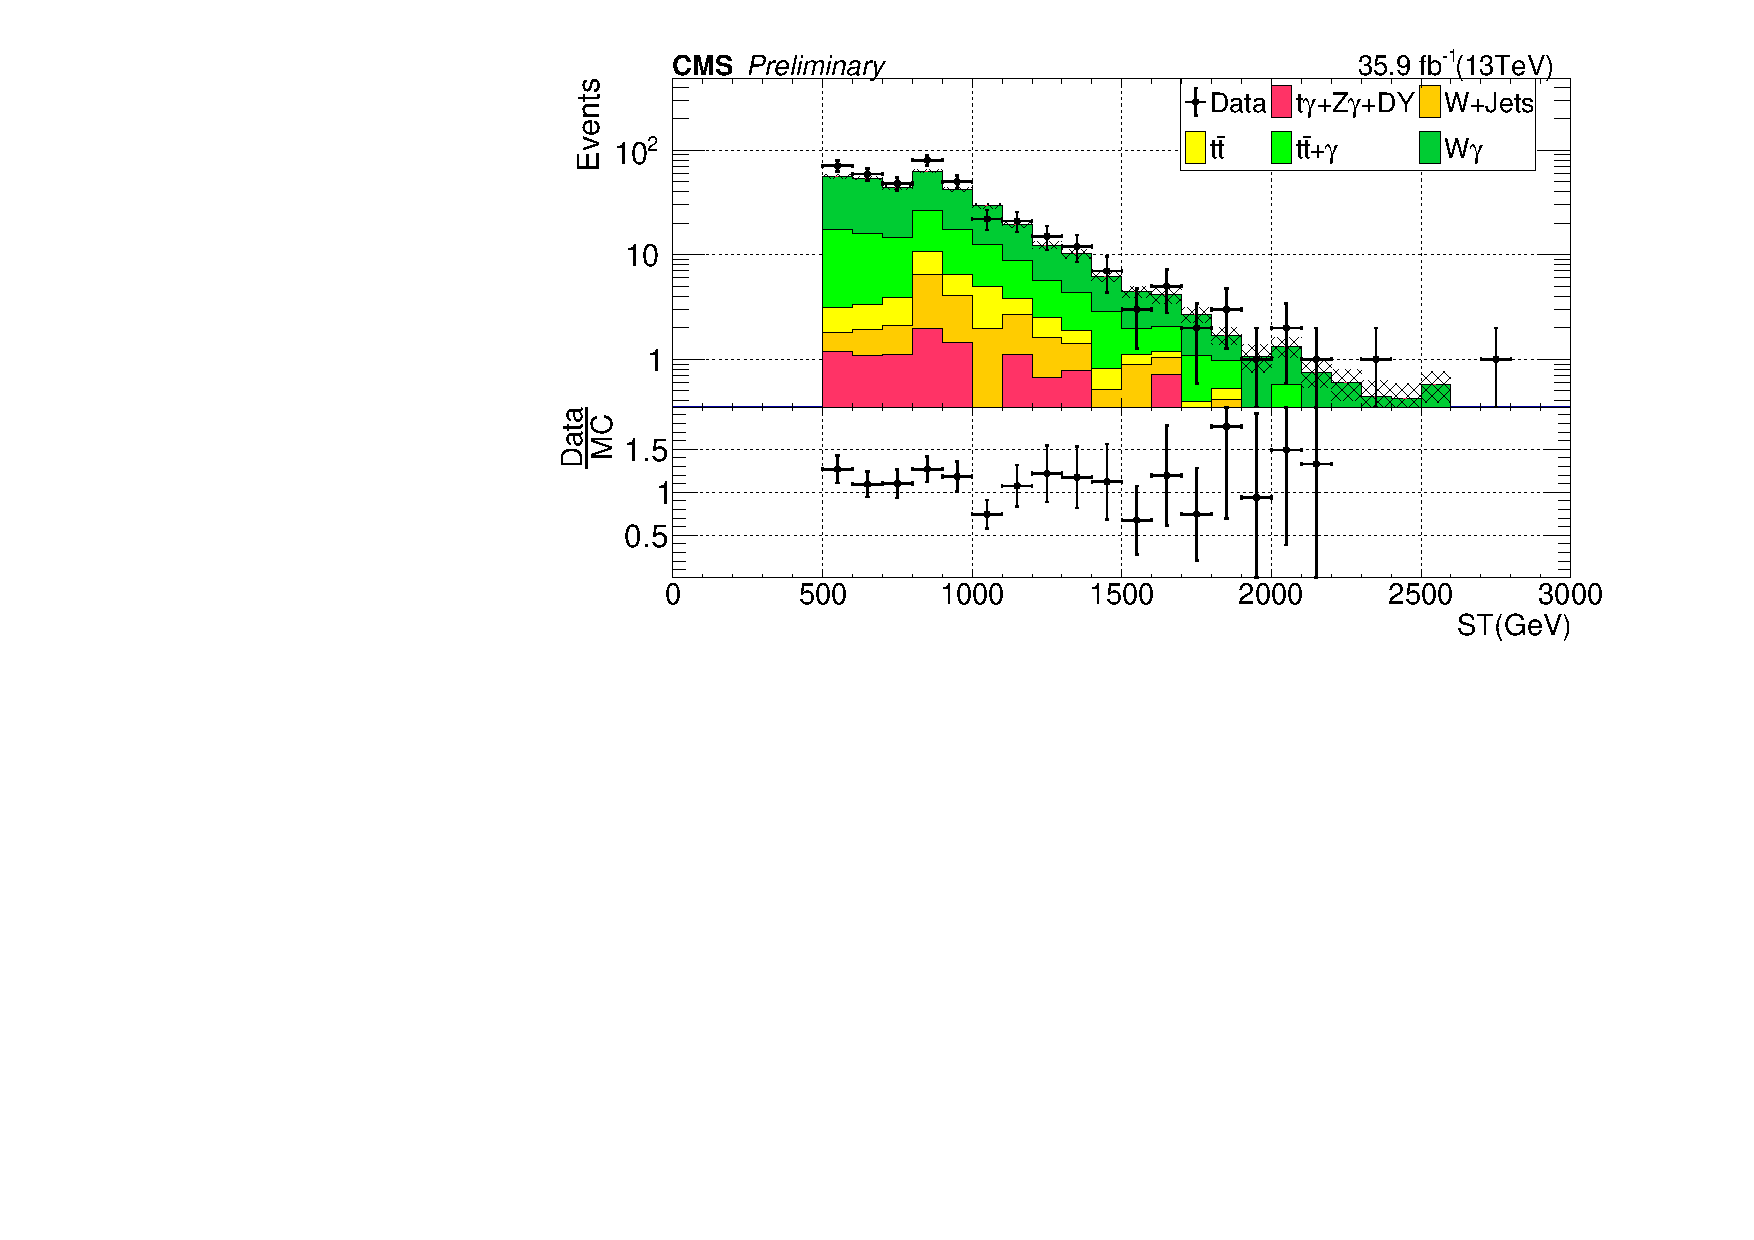
\includegraphics[width=0.48\linewidth]{../Figures/Chap3/lost_lepton/ST_Ele1.pdf}\\
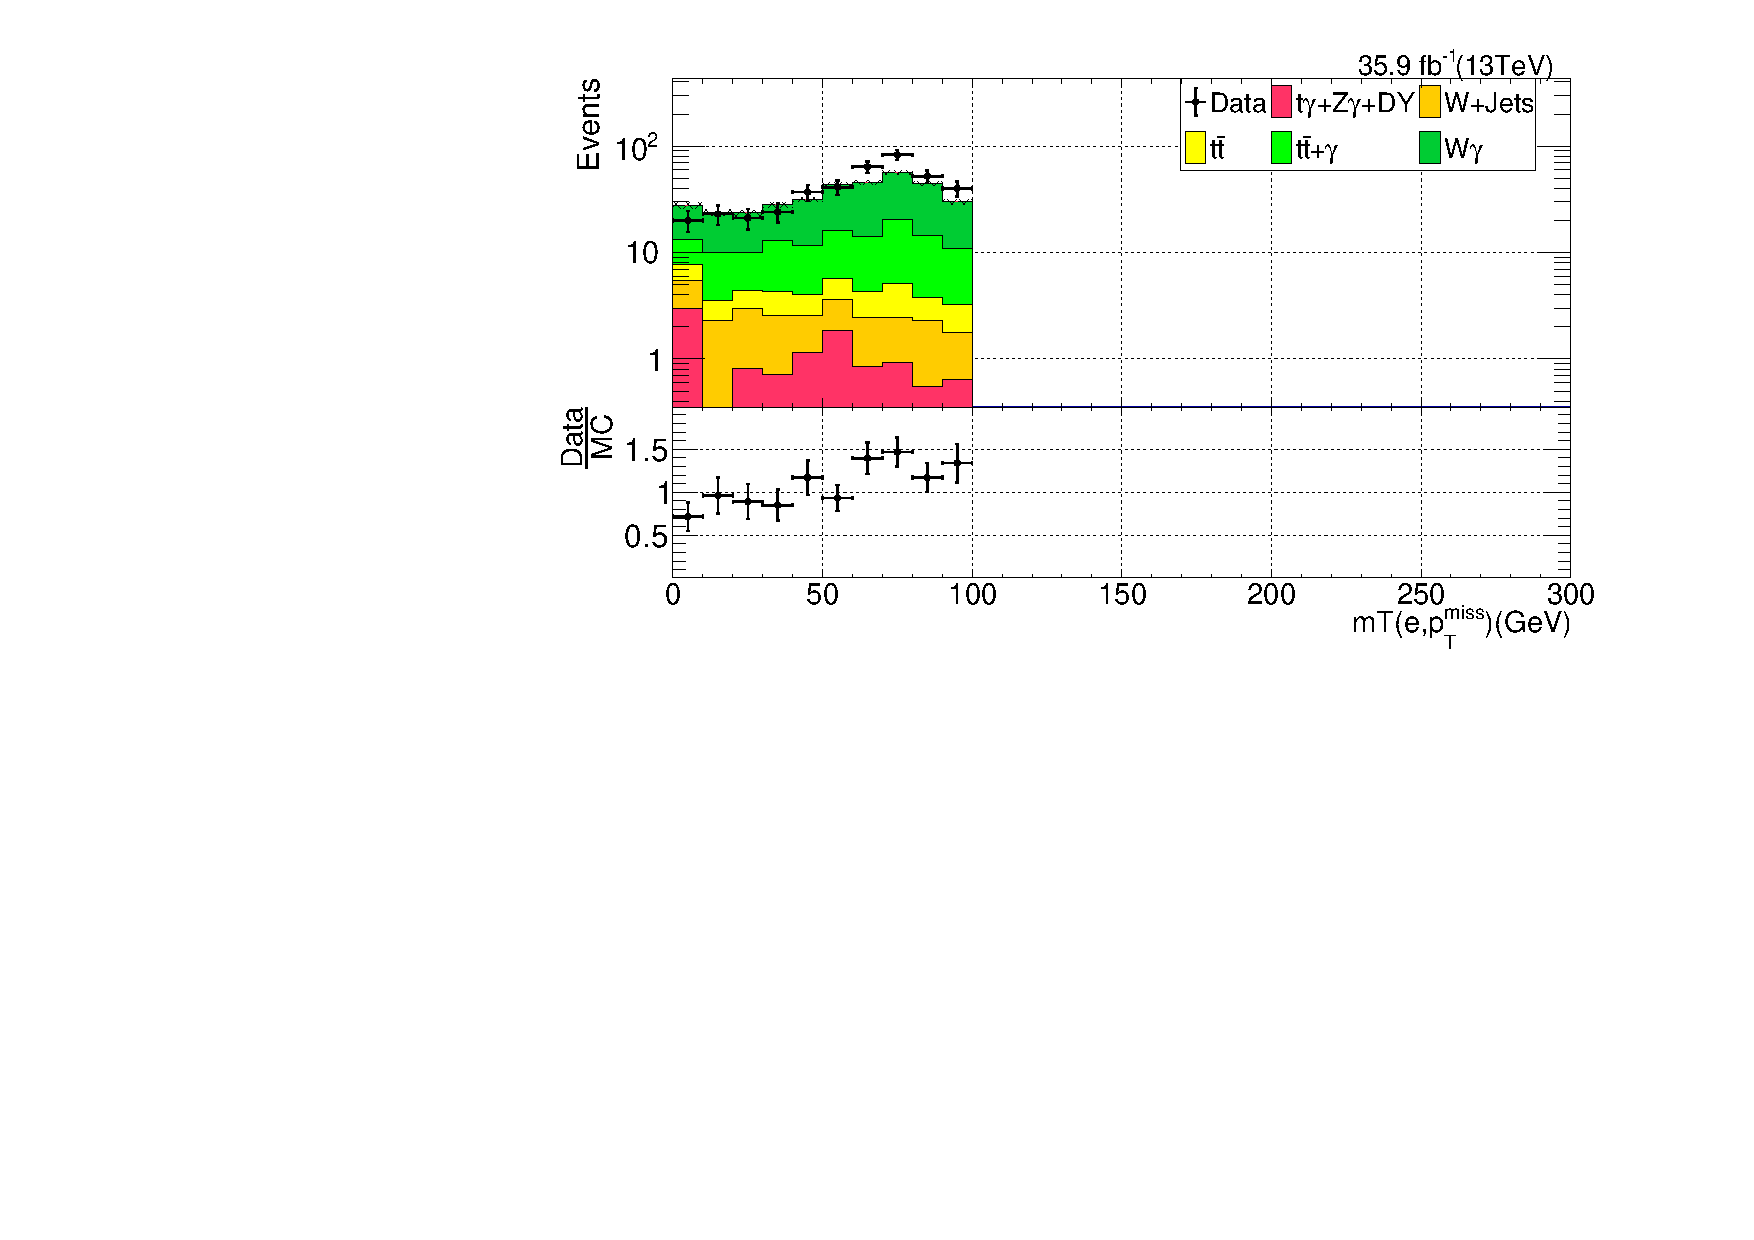
\includegraphics[width=0.48\linewidth]{../Figures/Chap3/lost_lepton/MT_Ele.pdf}
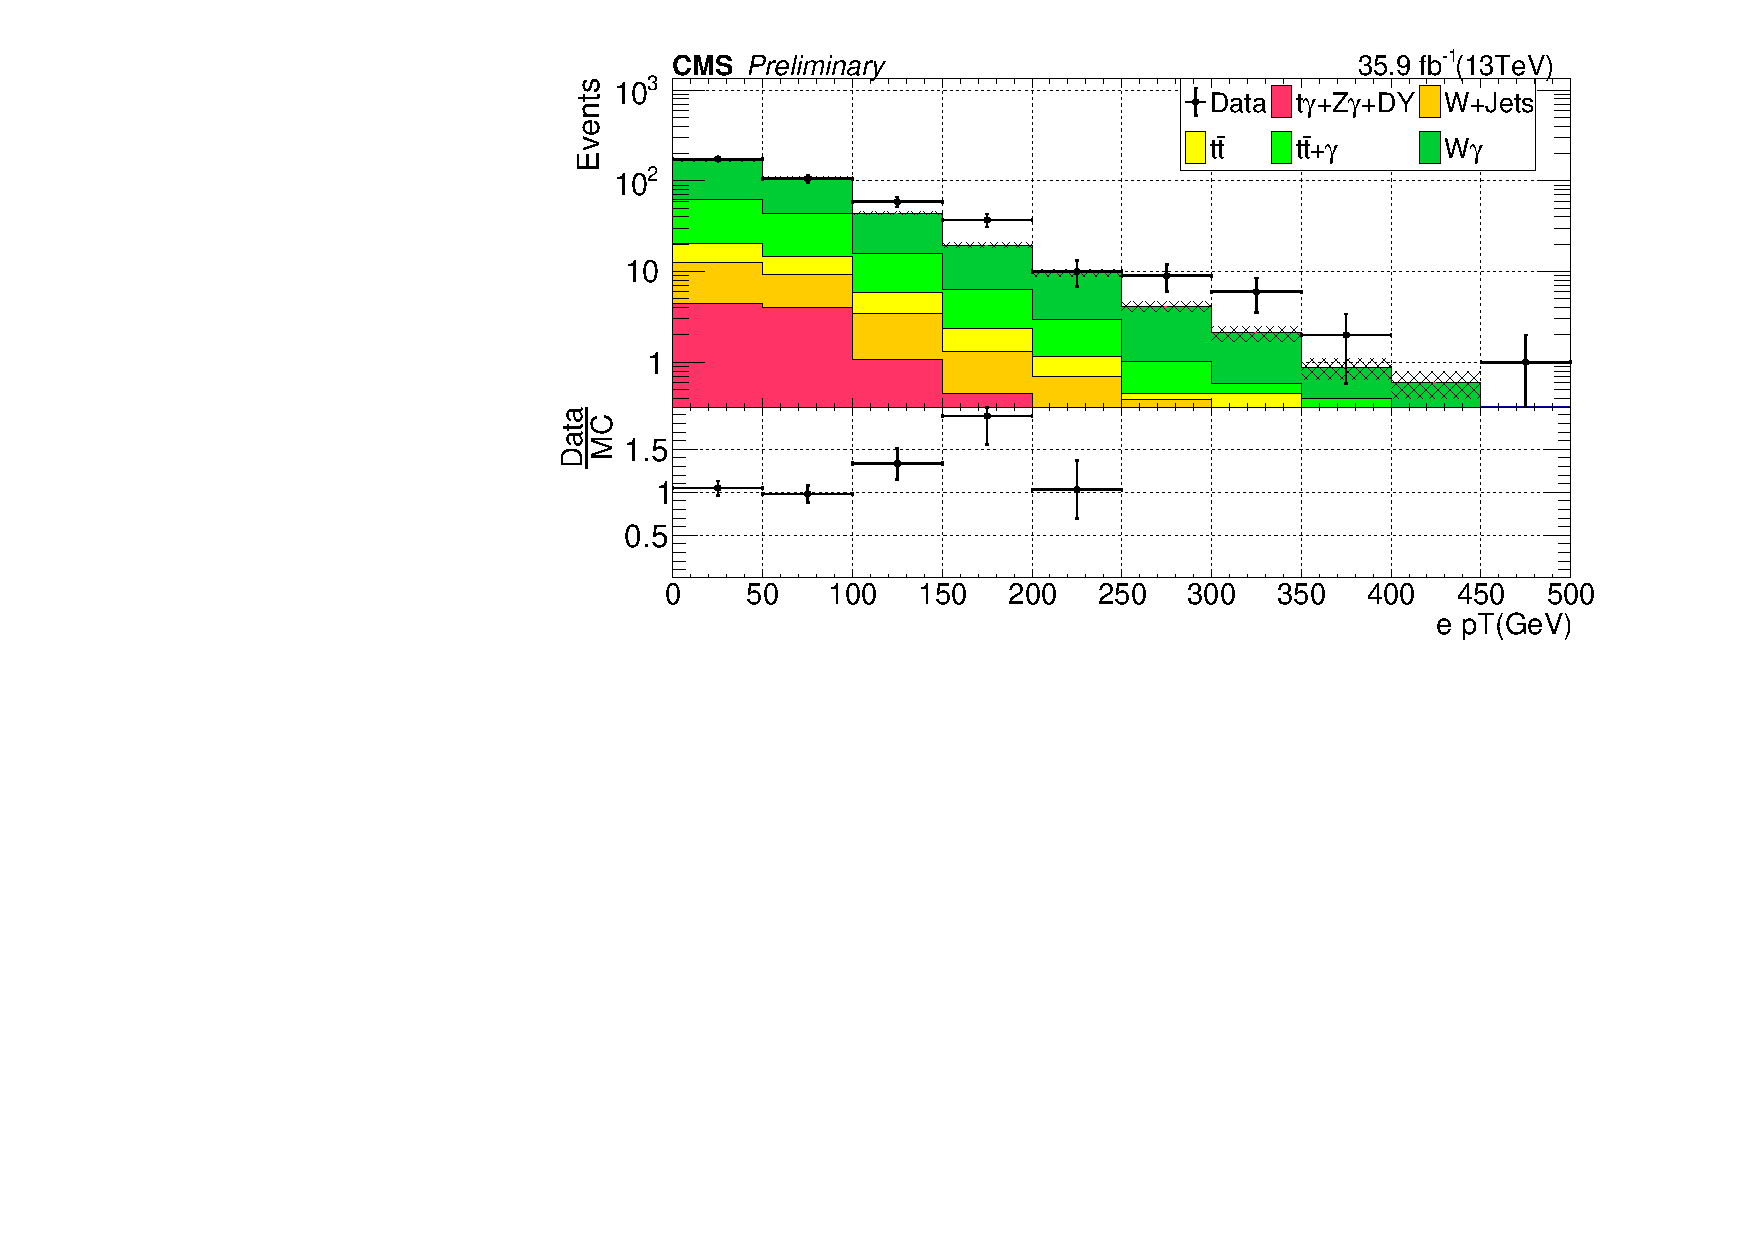
\includegraphics[width=0.48\linewidth]{../Figures/Chap3/lost_lepton/ElePt.pdf}\\
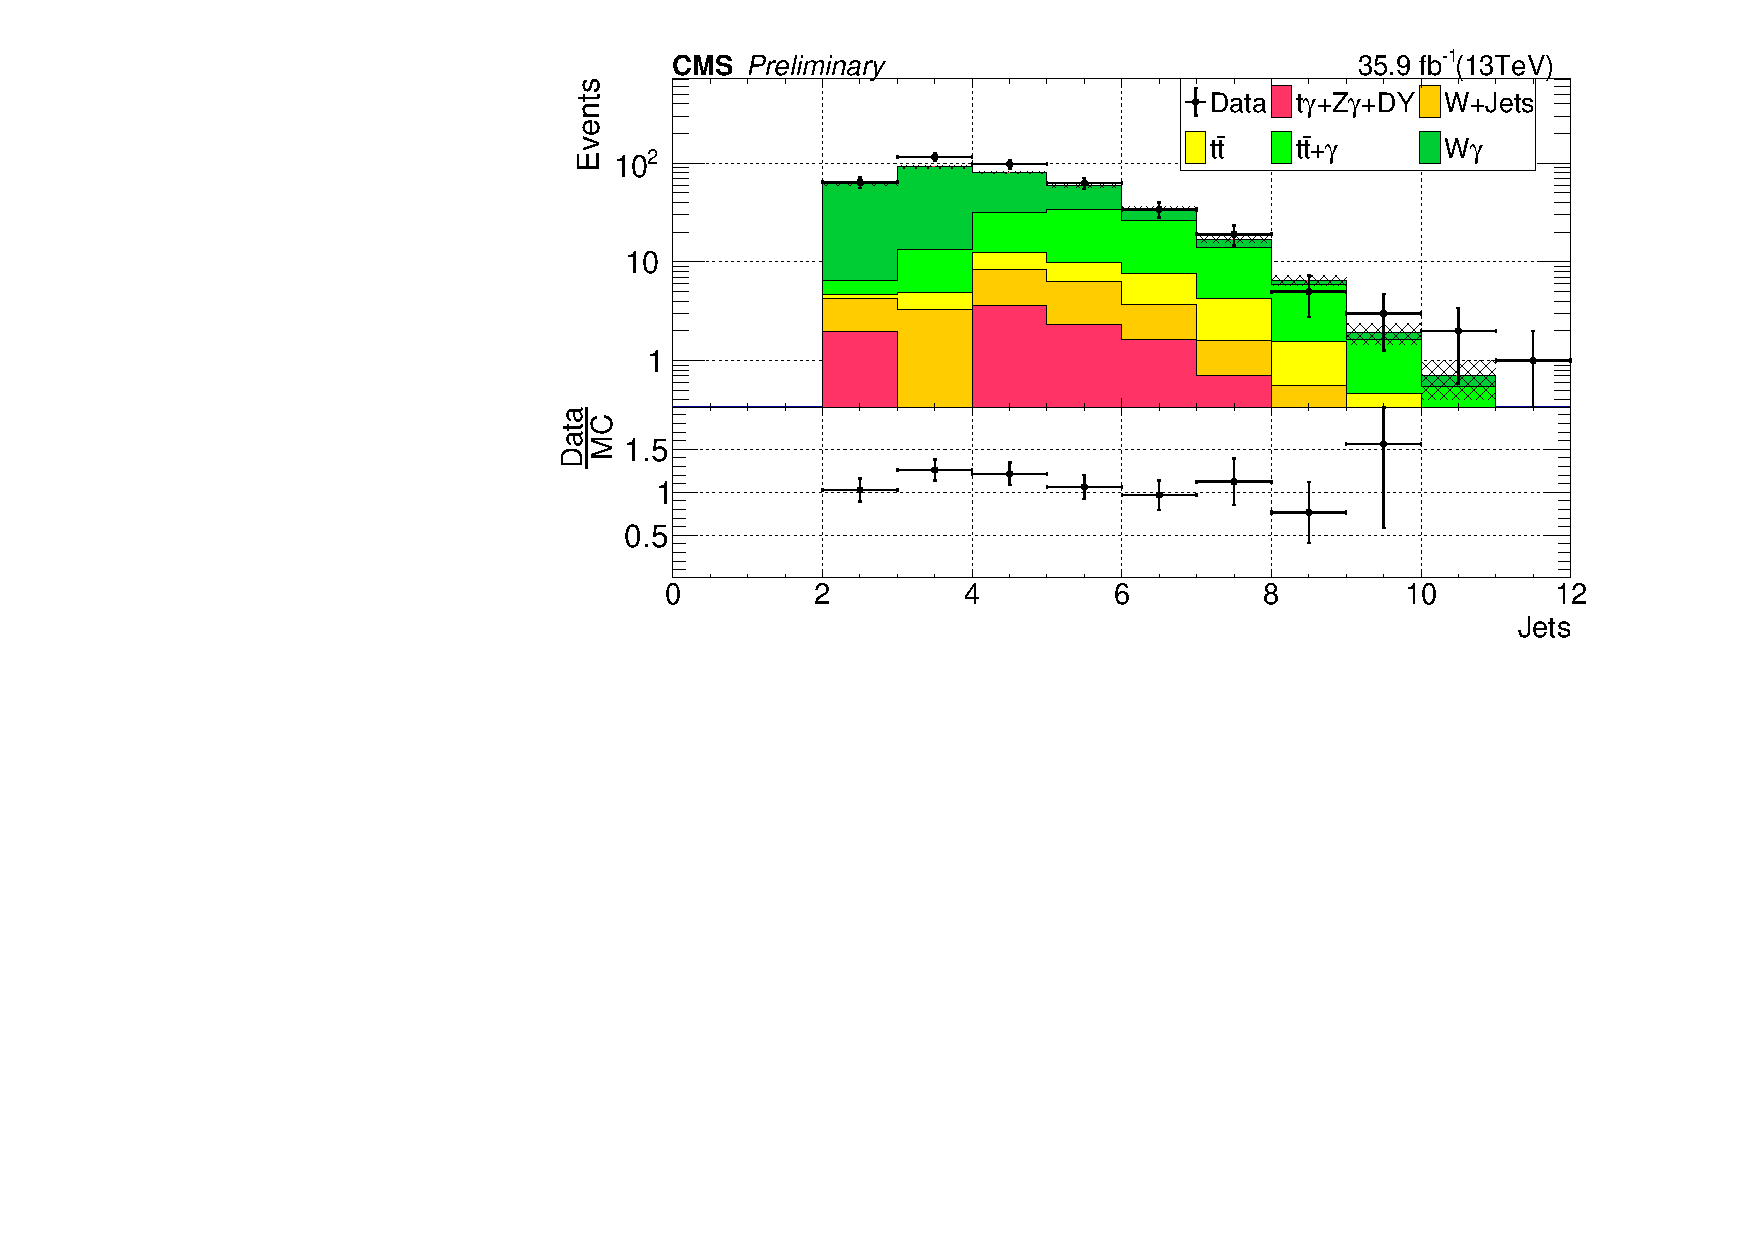
\includegraphics[width=0.48\linewidth]{../Figures/Chap3/lost_lepton/nHadJets_Ele1.pdf}
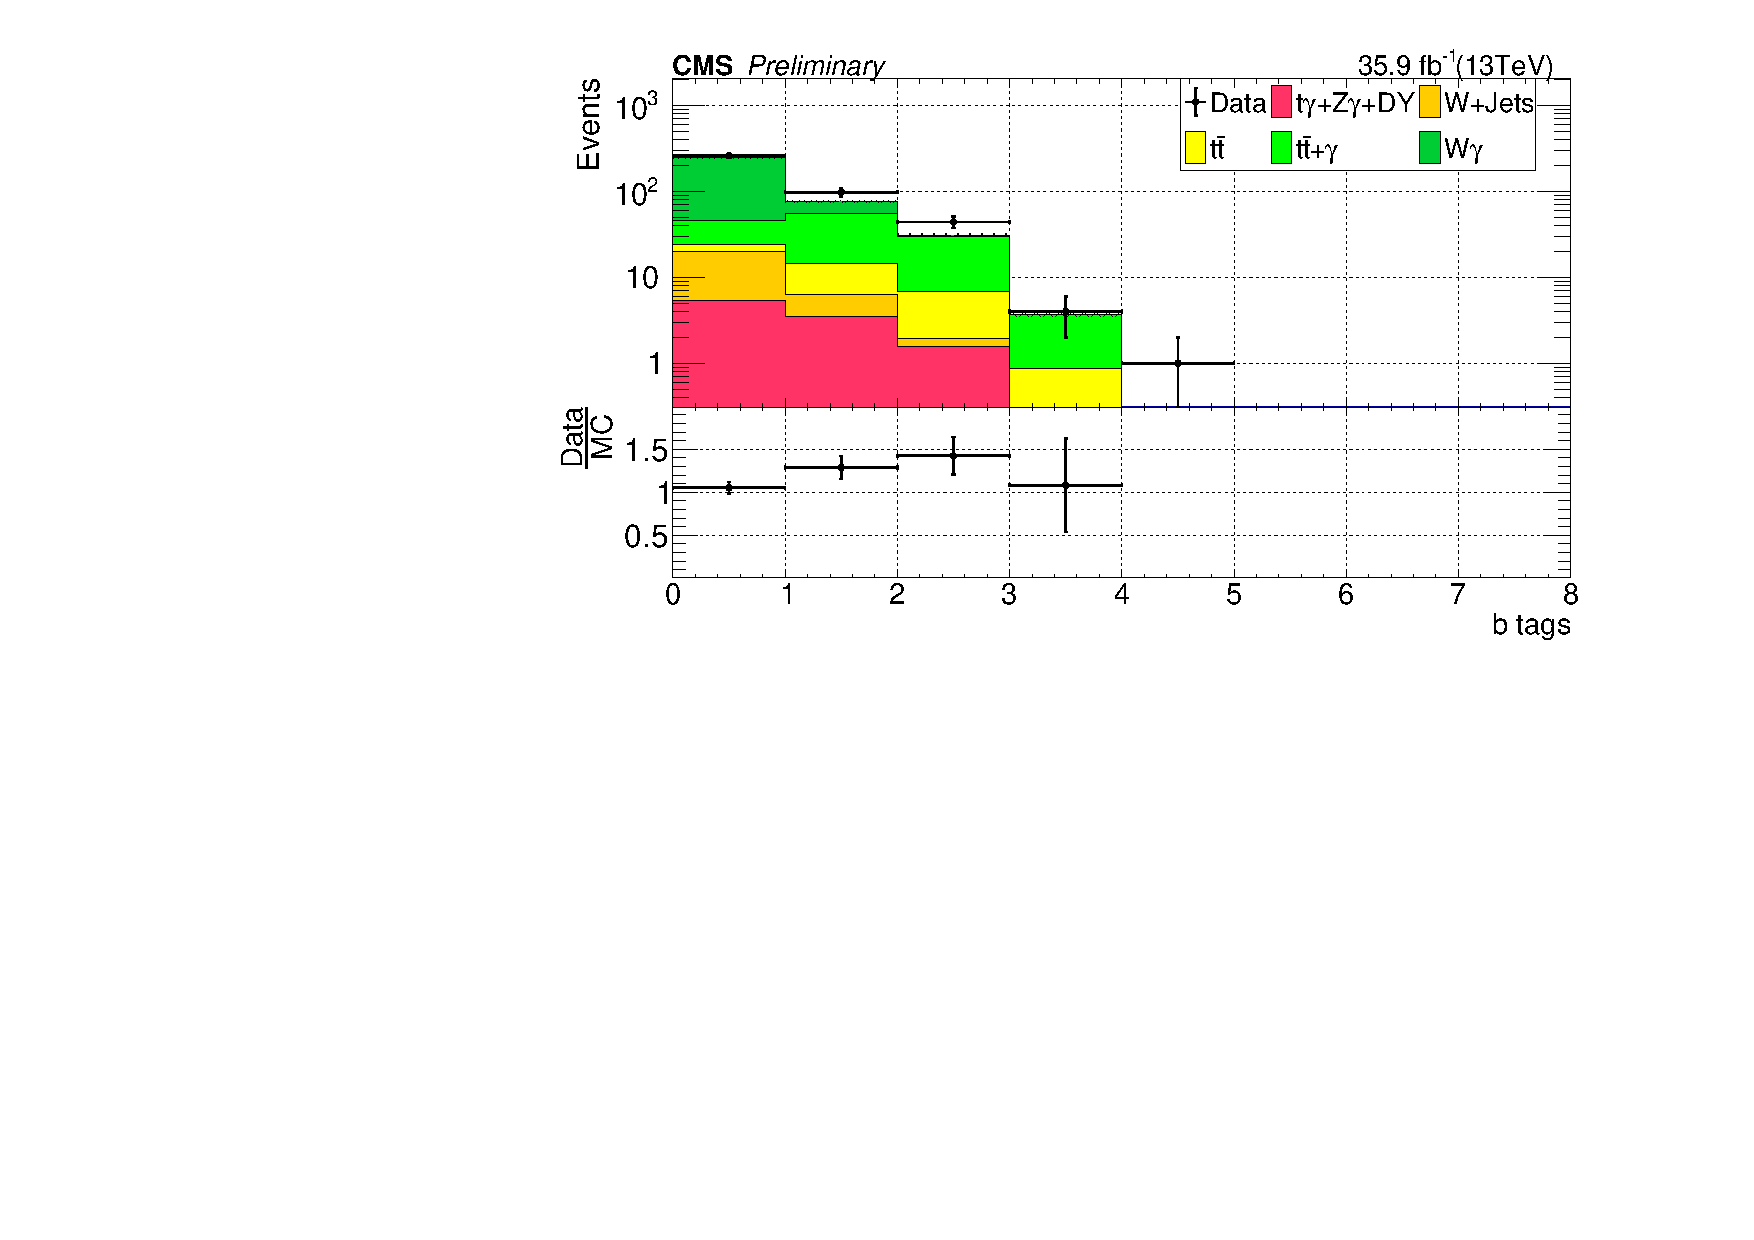
\includegraphics[width=0.48\linewidth]{../Figures/Chap3/lost_lepton/nBTags_Ele1.pdf}
\end{figure}


\begin{figure}[h!]
\centering
\caption[Data vs MC for $\mu\gamma$ CR]{Distribution of $\mu+\gamma$ events versus \ptmiss (top left), $S_T$ (top right), 
$M_T$ (middle left), $p_{T,\mu}$ (middle right), \nj (bottom left), \nb (bottom right).  
Filled histograms denoted expected yields from MC for various processes.  Markers represent data yields.
MC event yields are scaled to the same integrated luminosity as data.}
\label{fig:lost_mu_CR_dist}
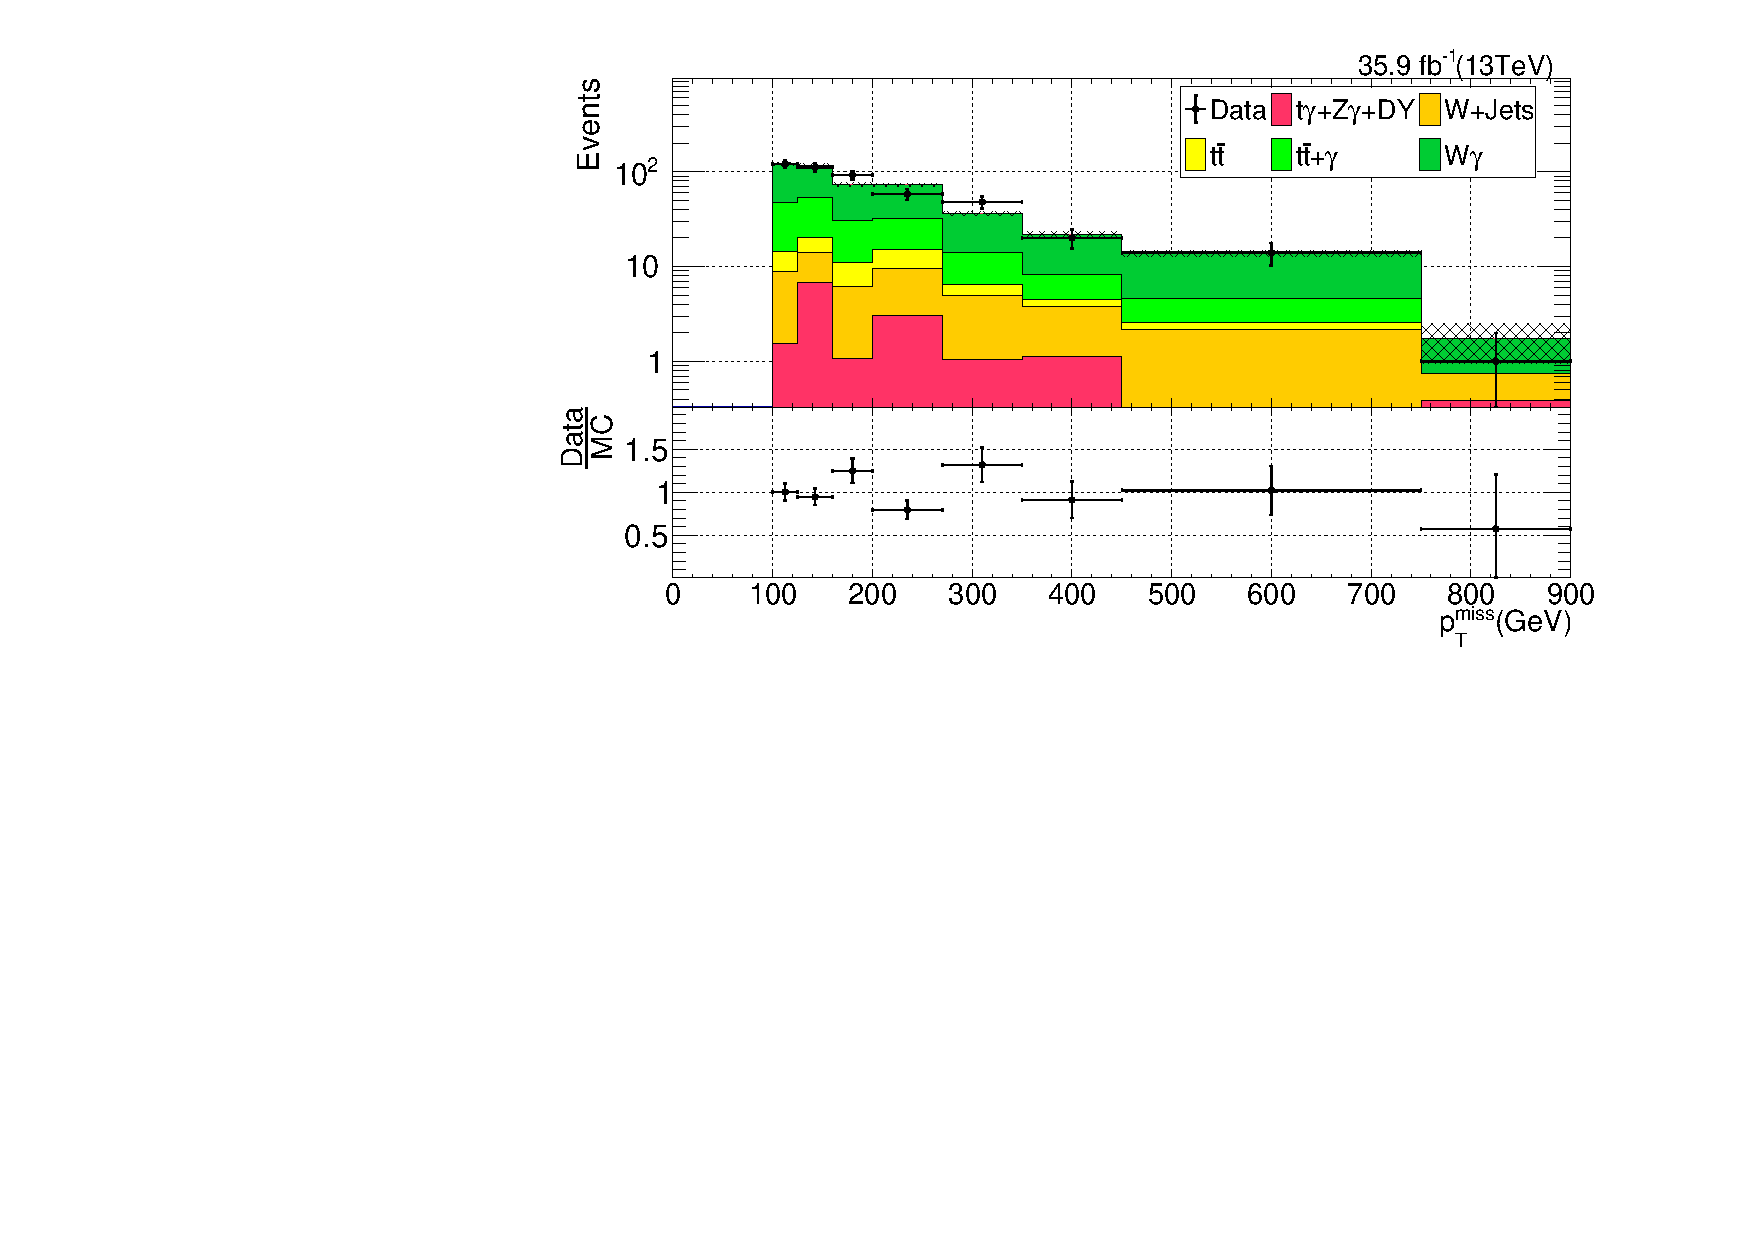
\includegraphics[width=0.48\linewidth]{../Figures/Chap3/lost_lepton/METvarBin_Mu1.pdf}
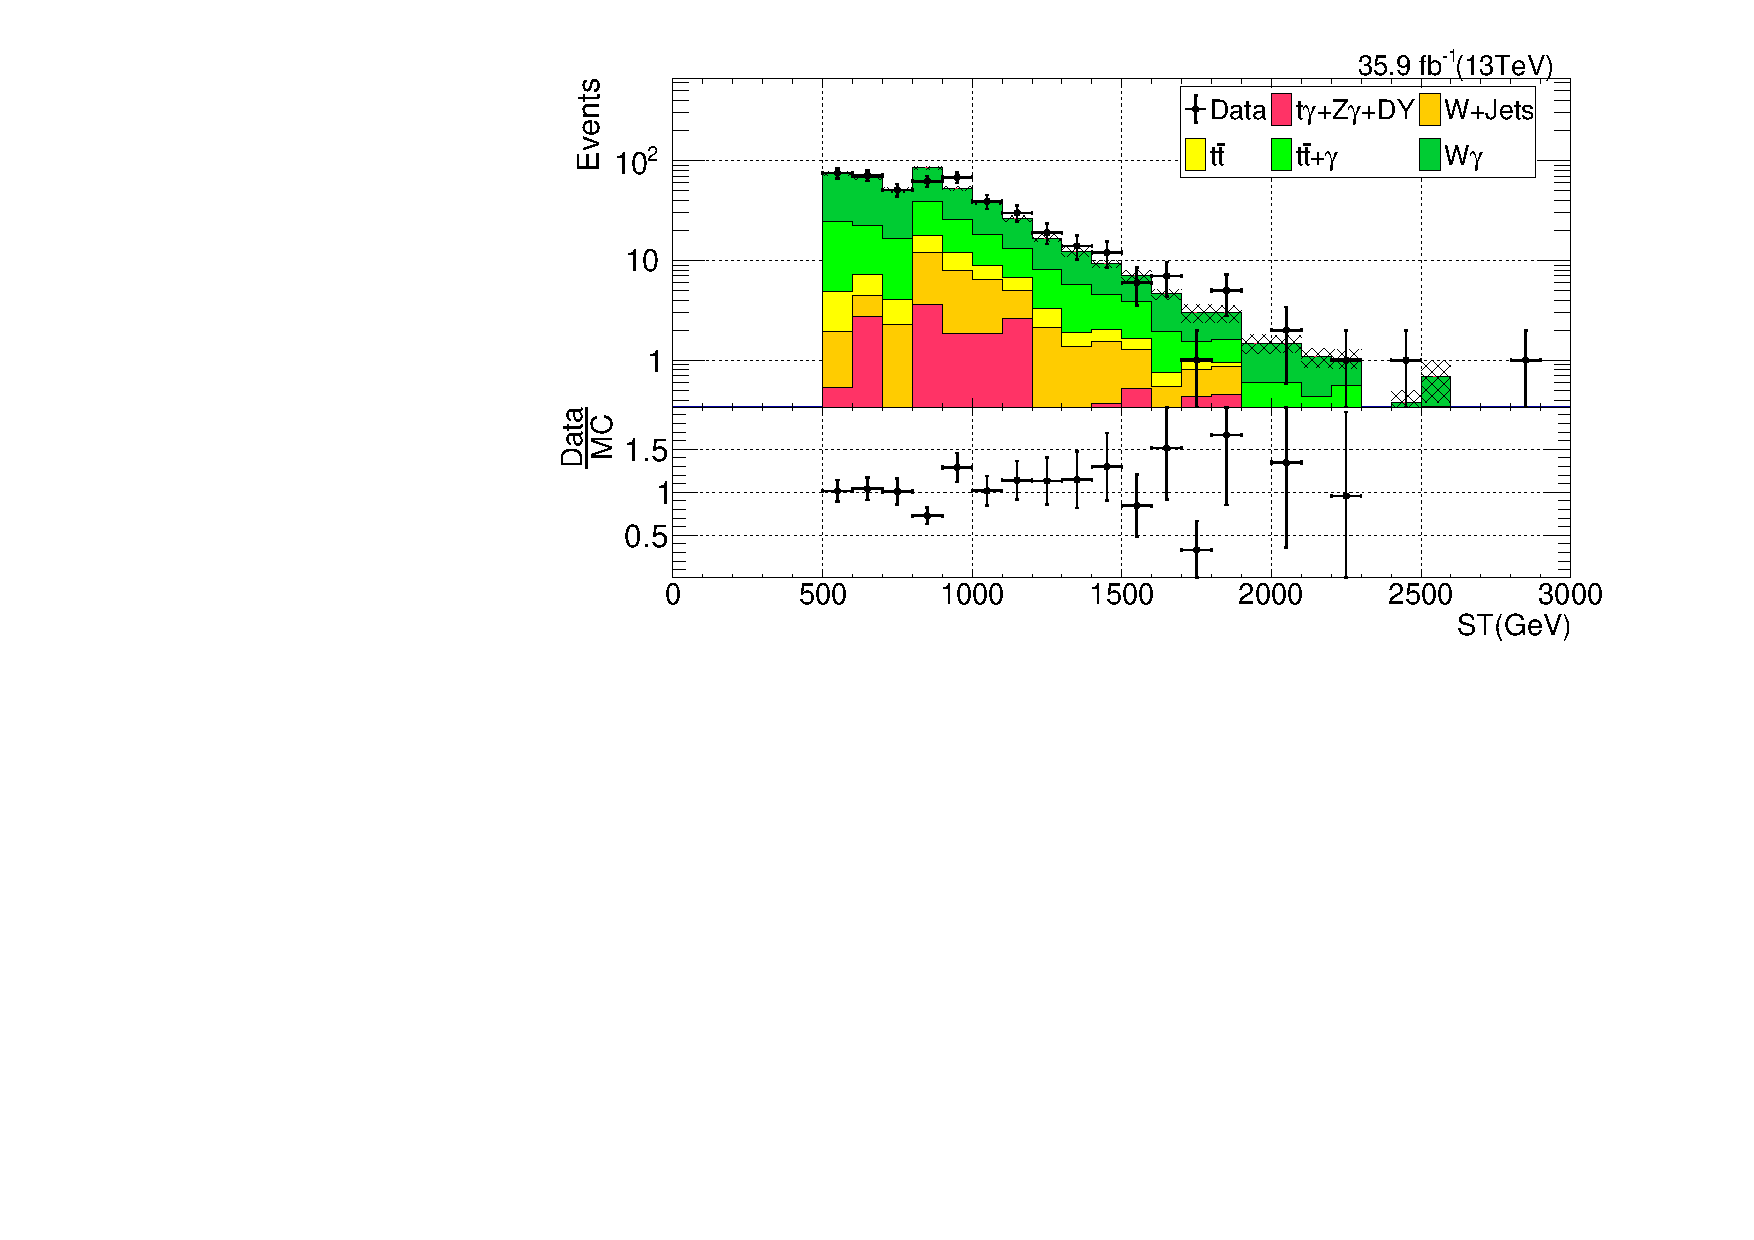
\includegraphics[width=0.48\linewidth]{../Figures/Chap3/lost_lepton/ST_Mu1.pdf}\\
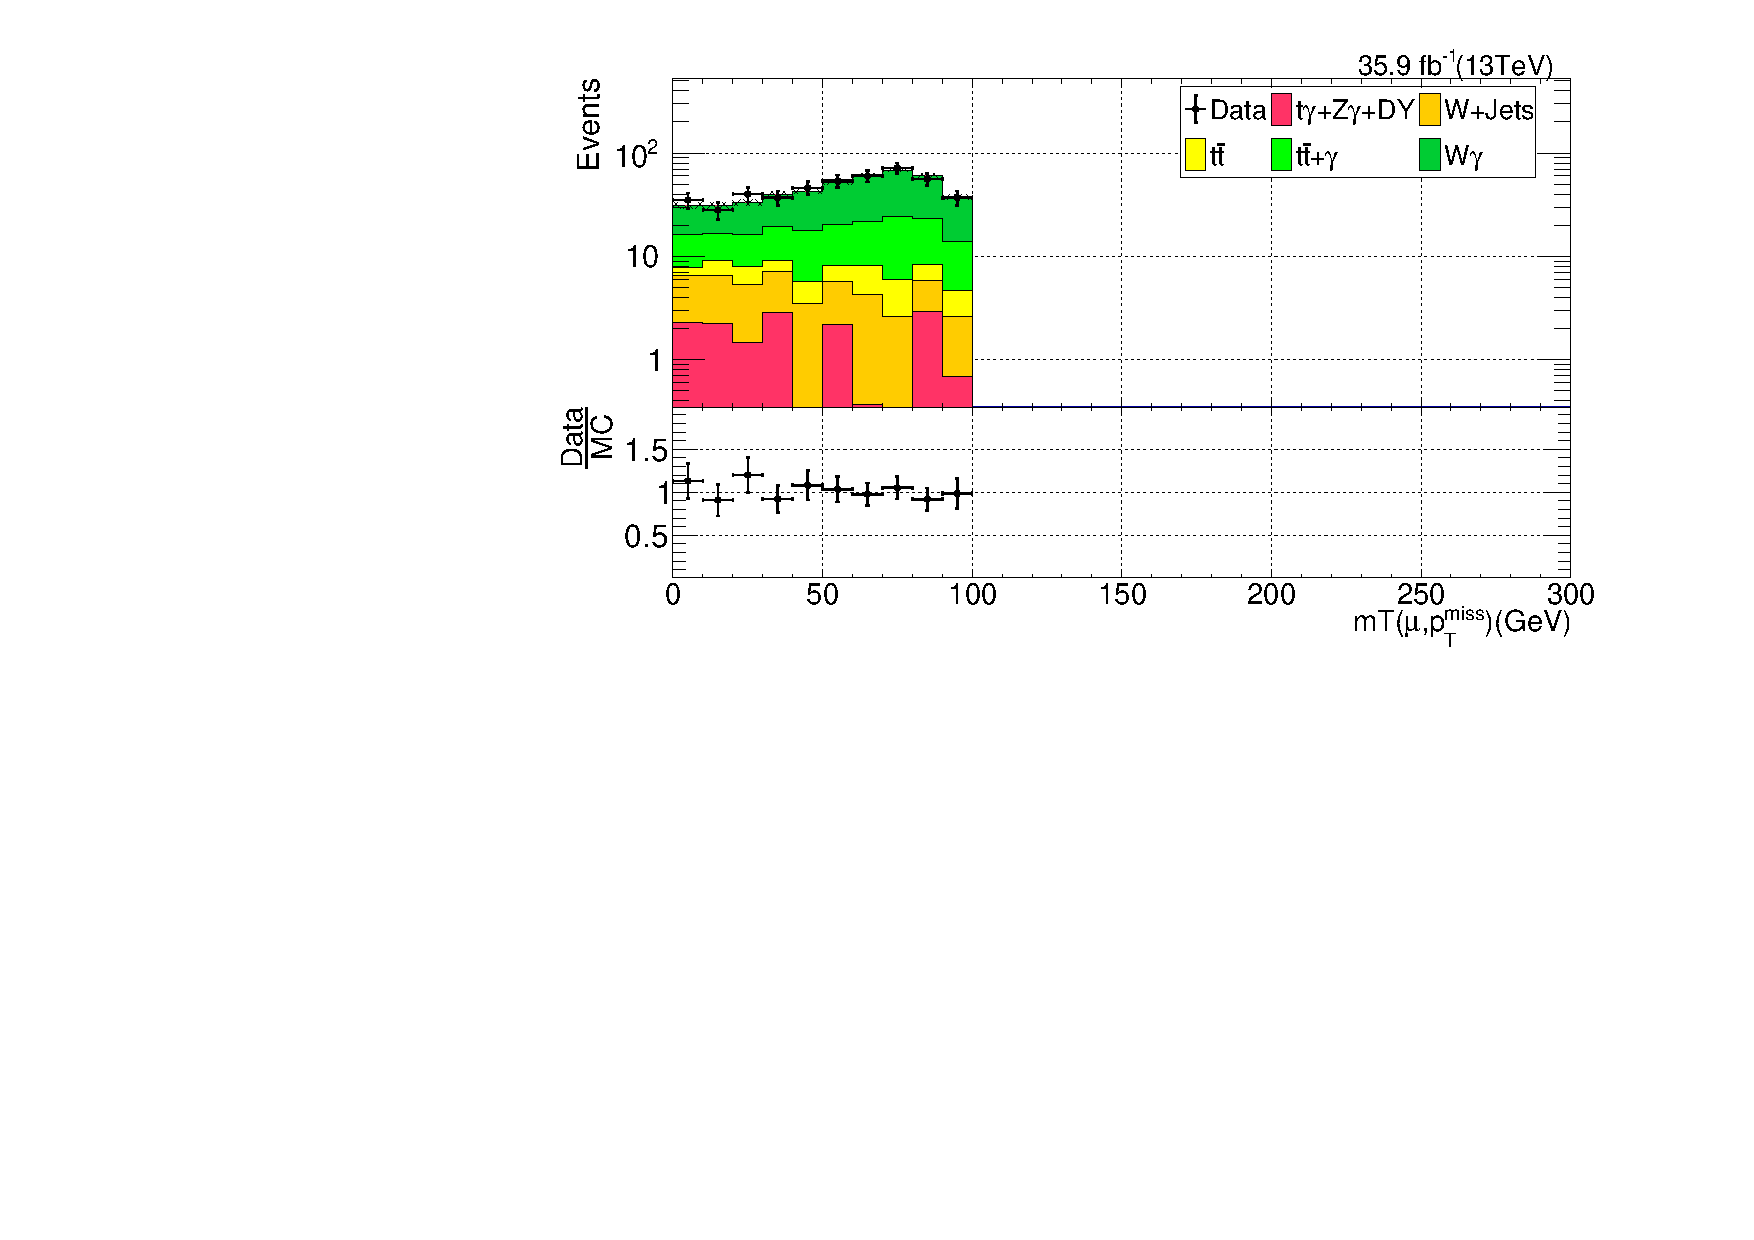
\includegraphics[width=0.48\linewidth]{../Figures/Chap3/lost_lepton/MT_Mu.pdf}
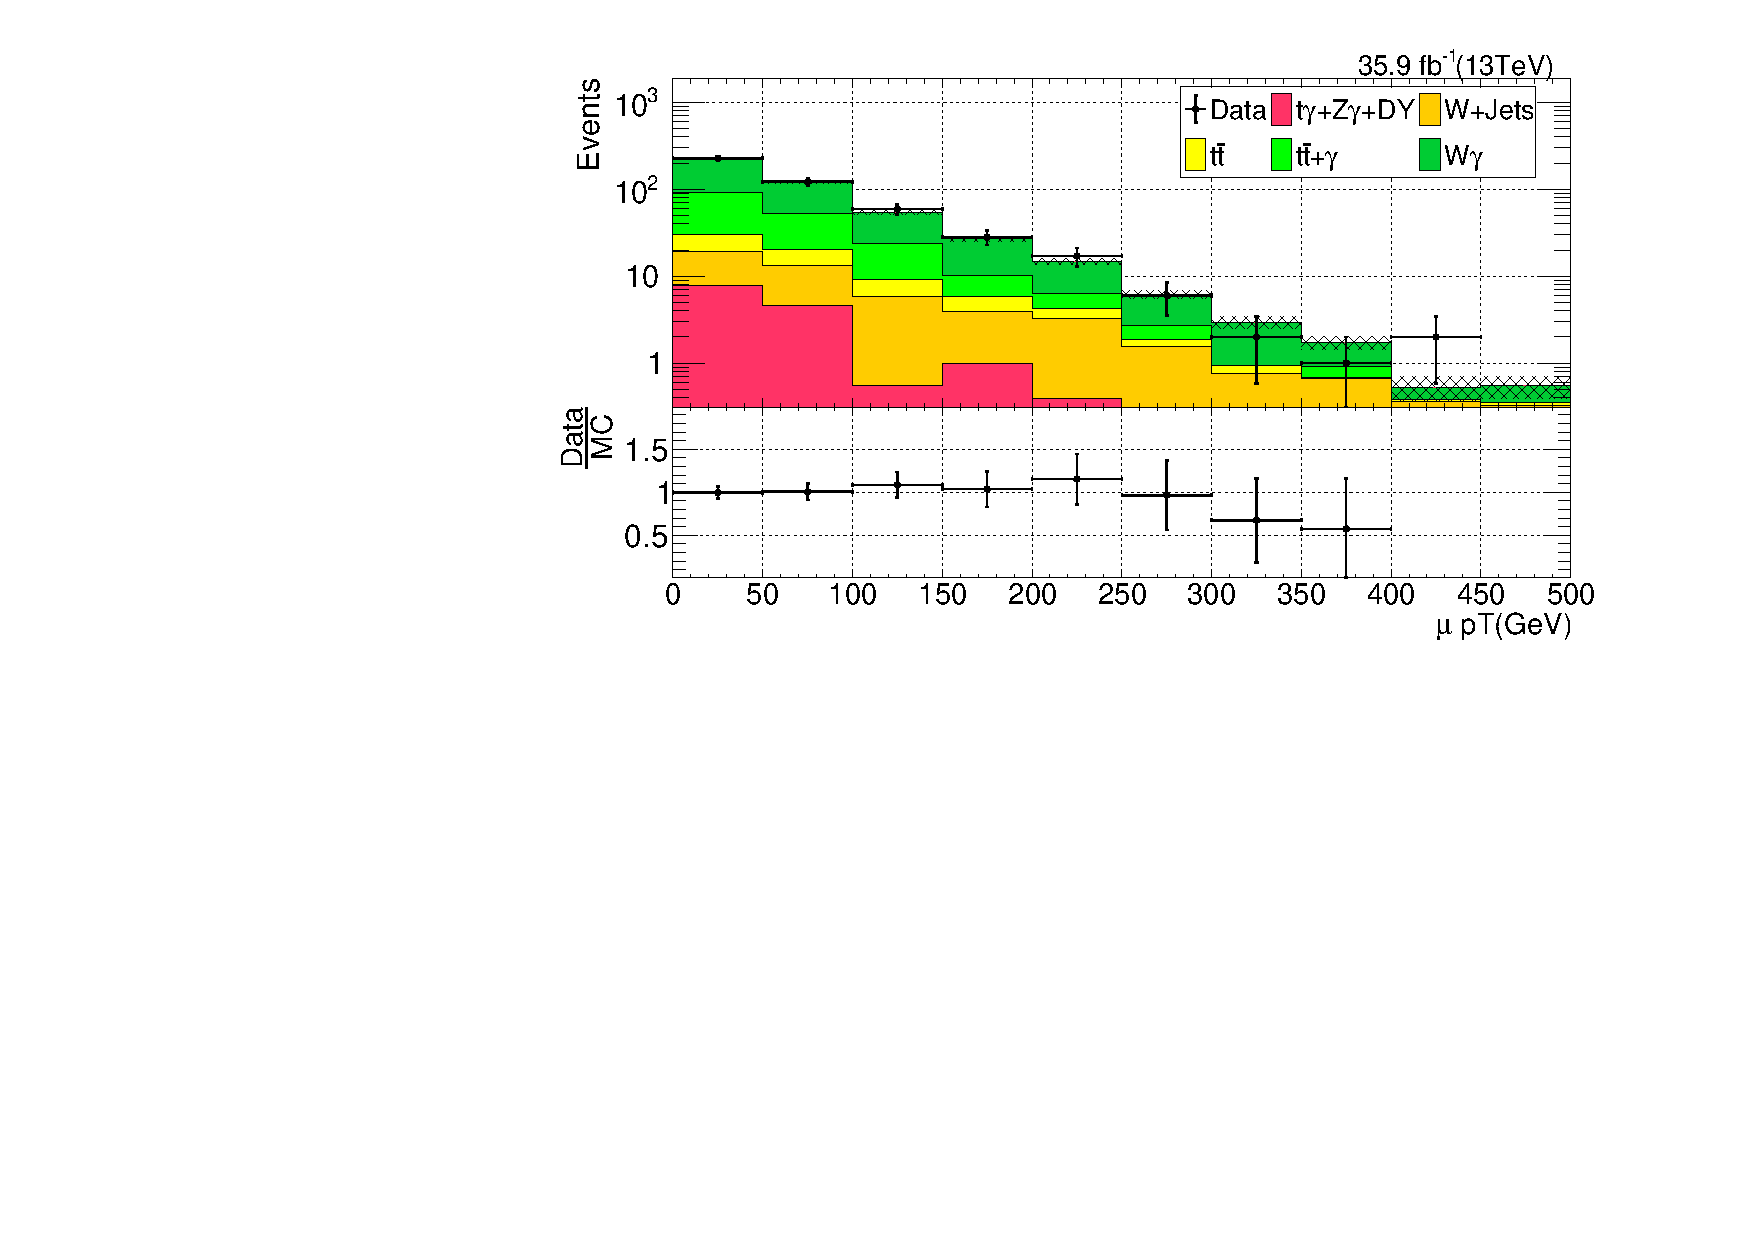
\includegraphics[width=0.48\linewidth]{../Figures/Chap3/lost_lepton/MuPt.pdf}\\
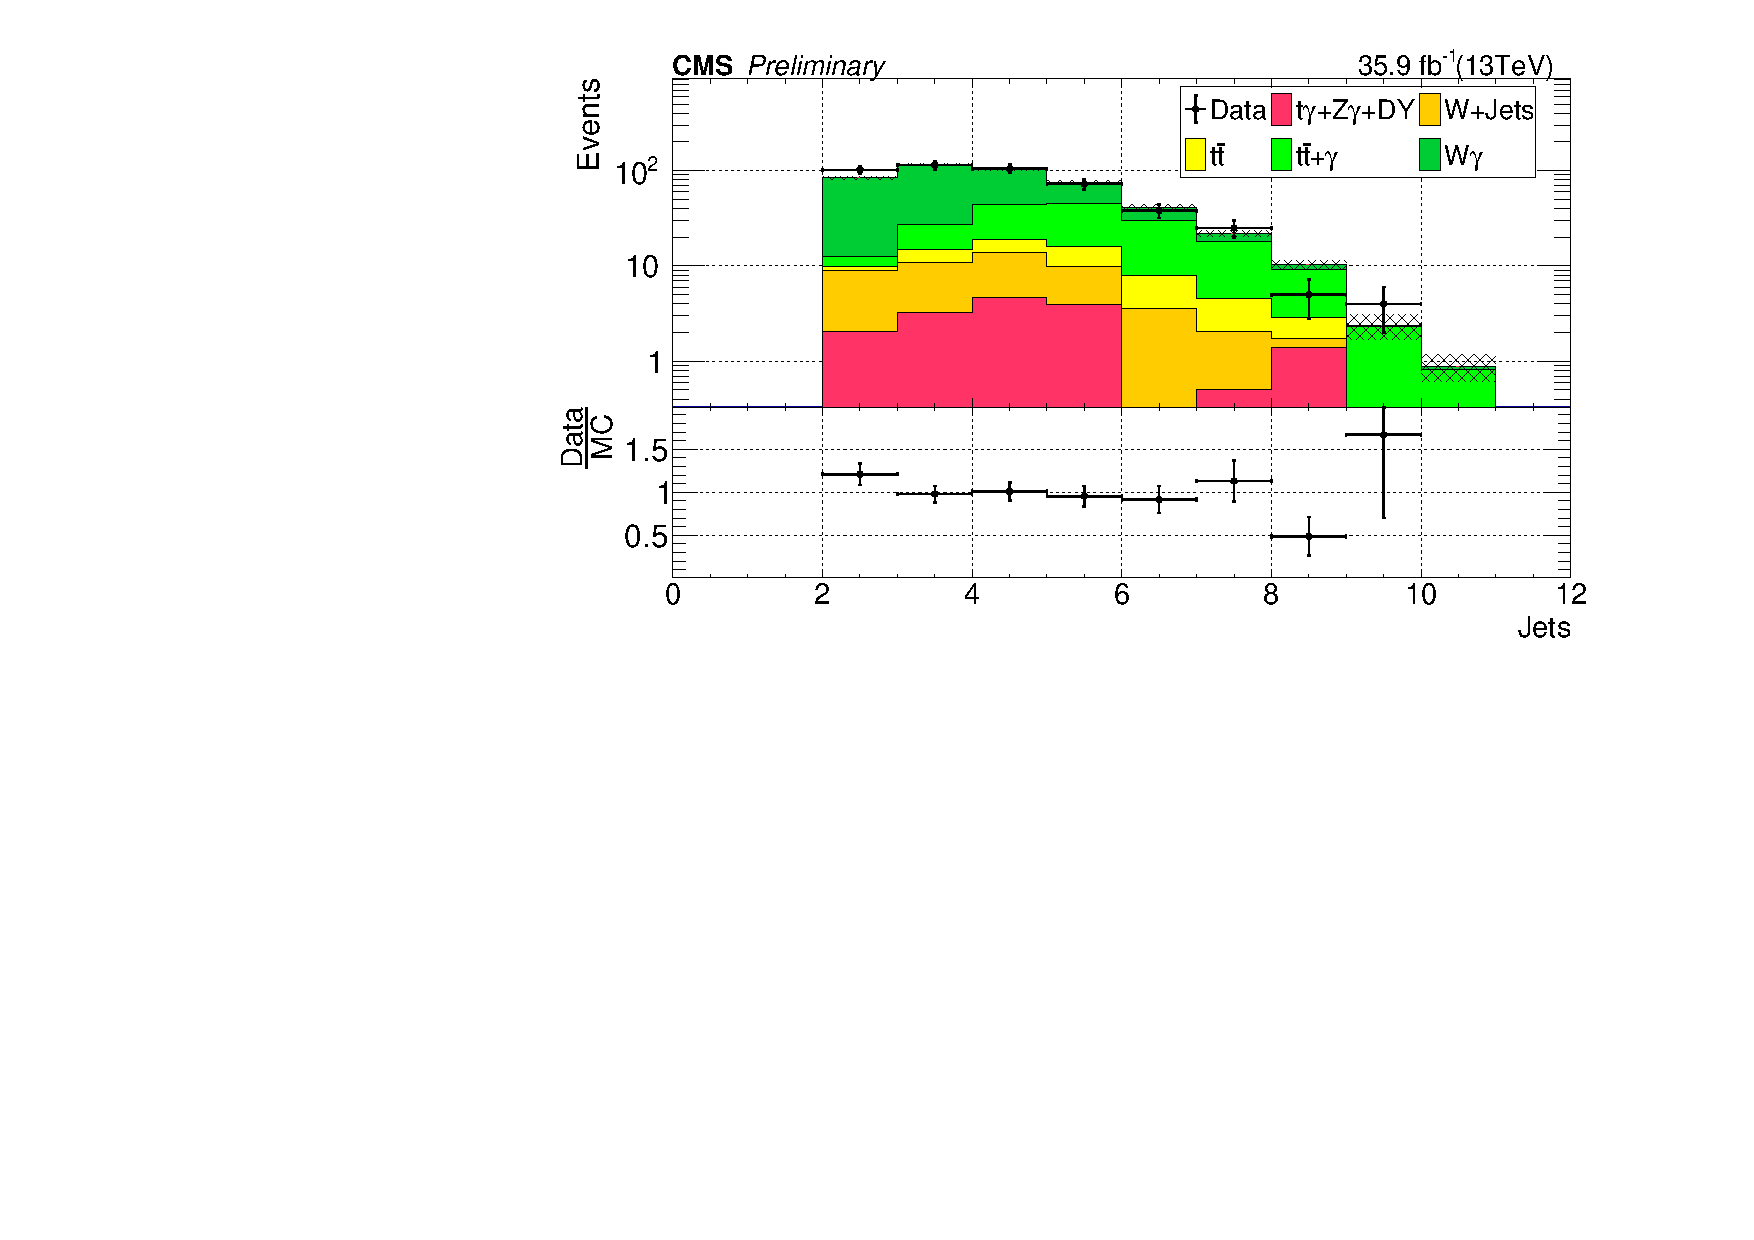
\includegraphics[width=0.48\linewidth]{../Figures/Chap3/lost_lepton/nHadJets_Mu1.pdf}
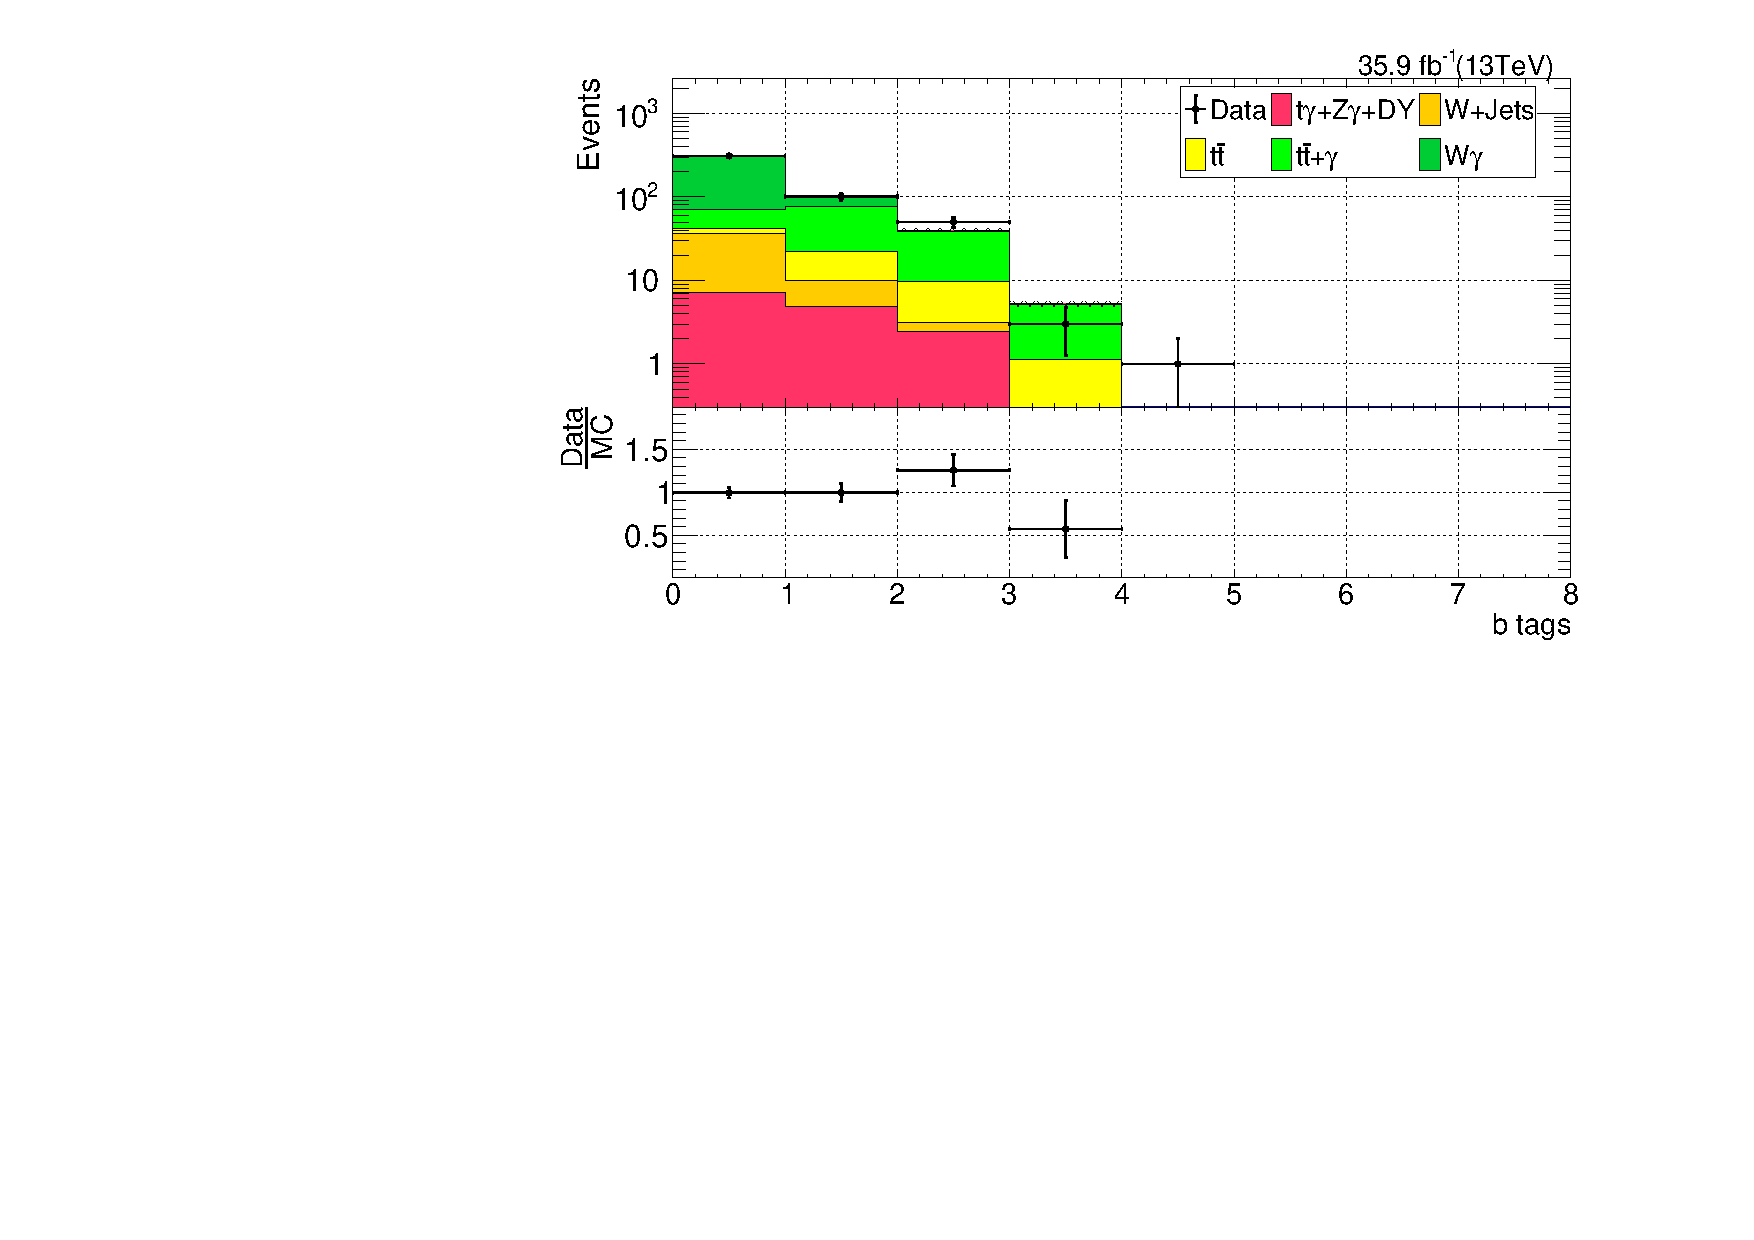
\includegraphics[width=0.48\linewidth]{../Figures/Chap3/lost_lepton/nBTags_Mu1.pdf}
\end{figure}

Comparisons of the observed yields and expected MC yields for the electron and muon control 
regions in Figures~\ref{fig:lost_mu_CR_dist} and~\ref{fig:lost_e_CR_dist}.  While the agreement between 
data and MC expectations is not directly required, MC modeling
of ratios of events can affect the lost lepton prediction.  Thus, data-MC comparisons of the
control region represent an important validation of the systematic uncertainties of the transfer
factors. 
MC modeling of the various analysis variables used to define the signal regions are generally 
found to have good agreement with data.  For the $e+\gamma$ CR the \pt, \ptmiss, and \mt
distributions are found to have differing shapes for data and MC. This could be because of some mis-modelling in the electron \pt and \ptmiss which affect \mt distibution since \mt is derived from \ptmiss and electron \pt. Effect of electron \pt mis-modeling can have maximum ~10\% effect on TF. Since the existing uncertainty on TF is 15-25\%, this systematic effect(if any) is already covered. In low \ptmiss bins(100-200 \gev), data-MC differences is found to be ~20\%. The low \ptmiss region is used as a sideband for multijet estimation and it does not correspond to any signal region. Lost electron contribution is very negligible in this sideband and it is dominated by multijet. So these differences are going to have very small effect (1-2\% or less) on multijet prediction.

All yields are computed after applying the b-tagging scale factors~\cite{BTV-16-002} and 
lepton scale factors to MC. 

\section{Z($\ell\ell$)+$\gamma$ control region}
A comparison of $ll+\gamma$ events in data with MC is shown in figure \ref{fig:llGammaDataMC}. In top left plot, since di-lepton pair is ignored, pT of the pair contributes to \ptmiss. Data agrees well with MC, within the statistical uncertainties.
\begin{figure}[h!]
\centering
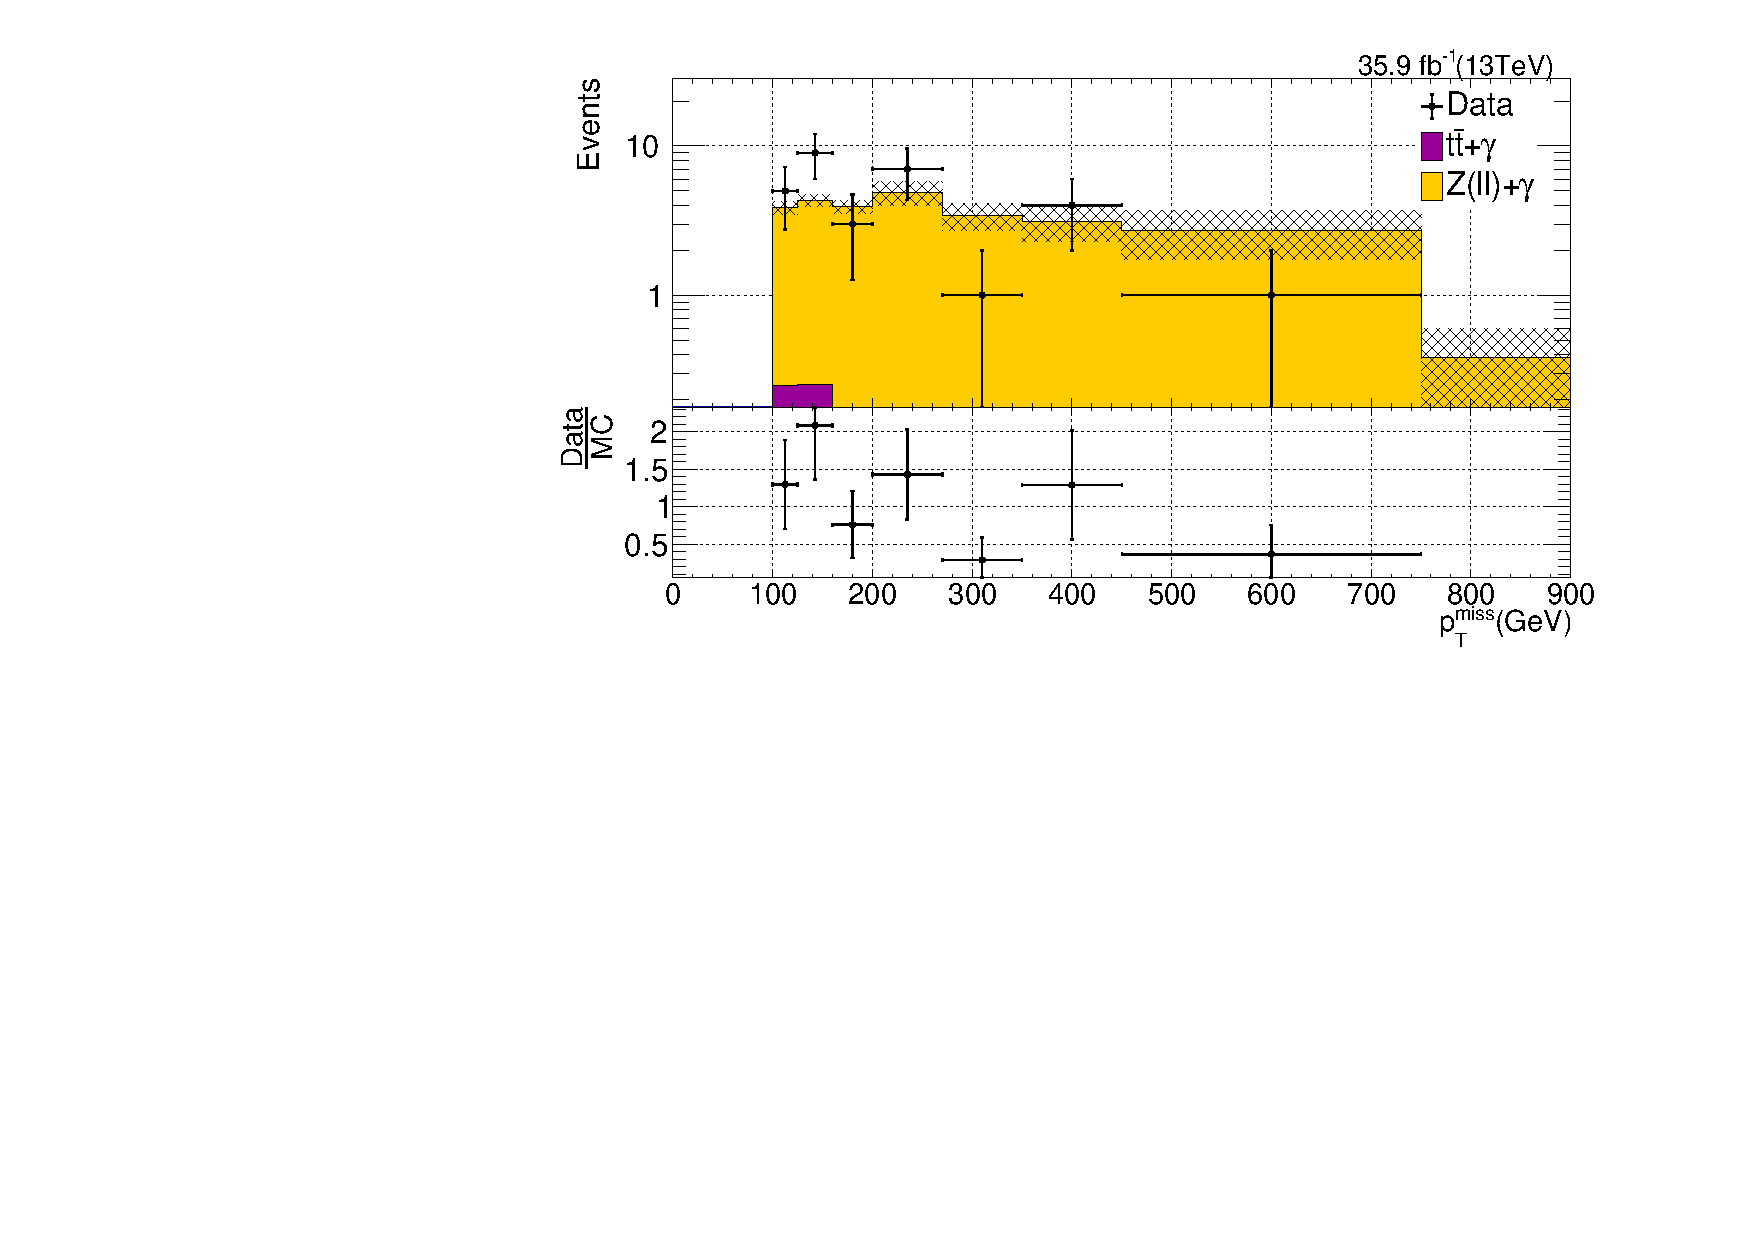
\includegraphics[width=0.48\linewidth]{../Figures/Chap3/zgamma/METvarBin_LLGDataMC.pdf}
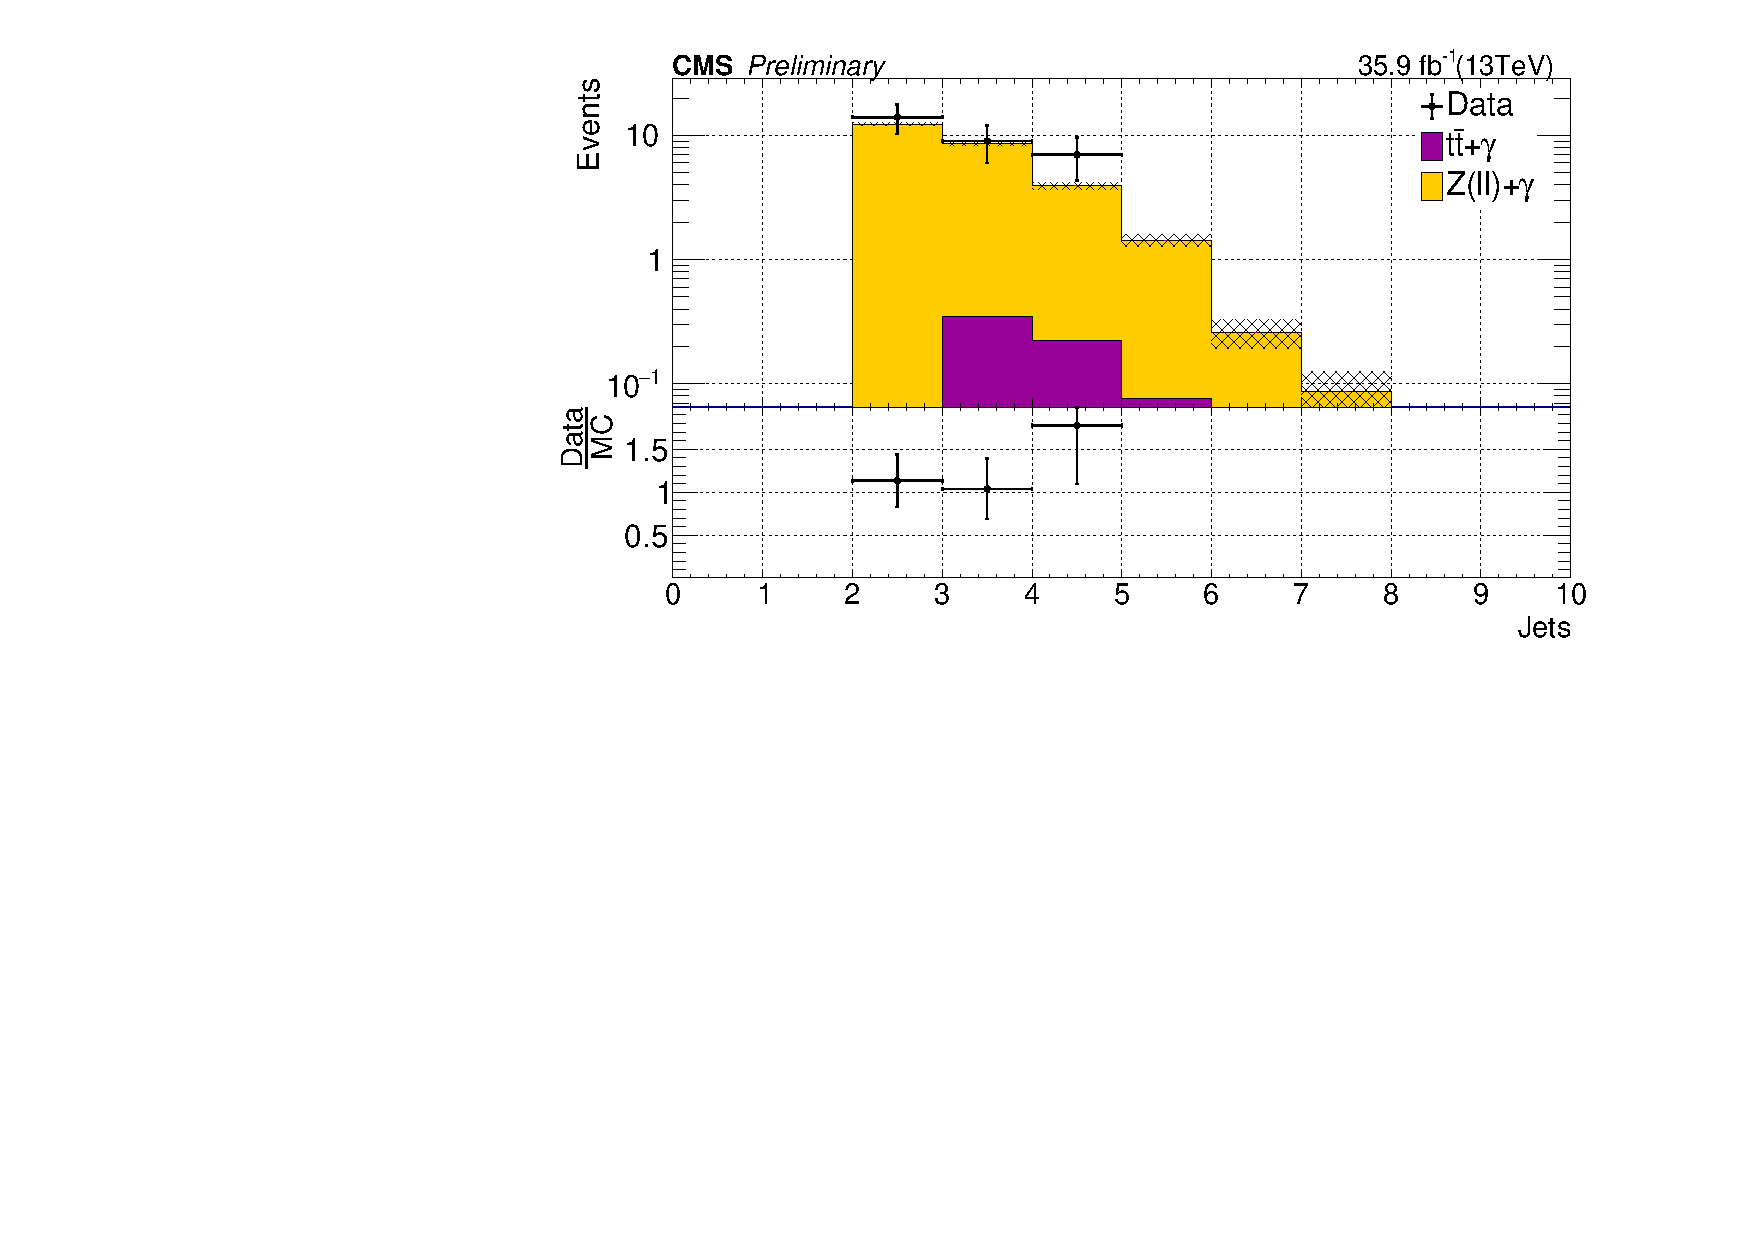
\includegraphics[width=0.48\linewidth]{../Figures/Chap3/zgamma/nHadJets_LLGDataMC.pdf}\\
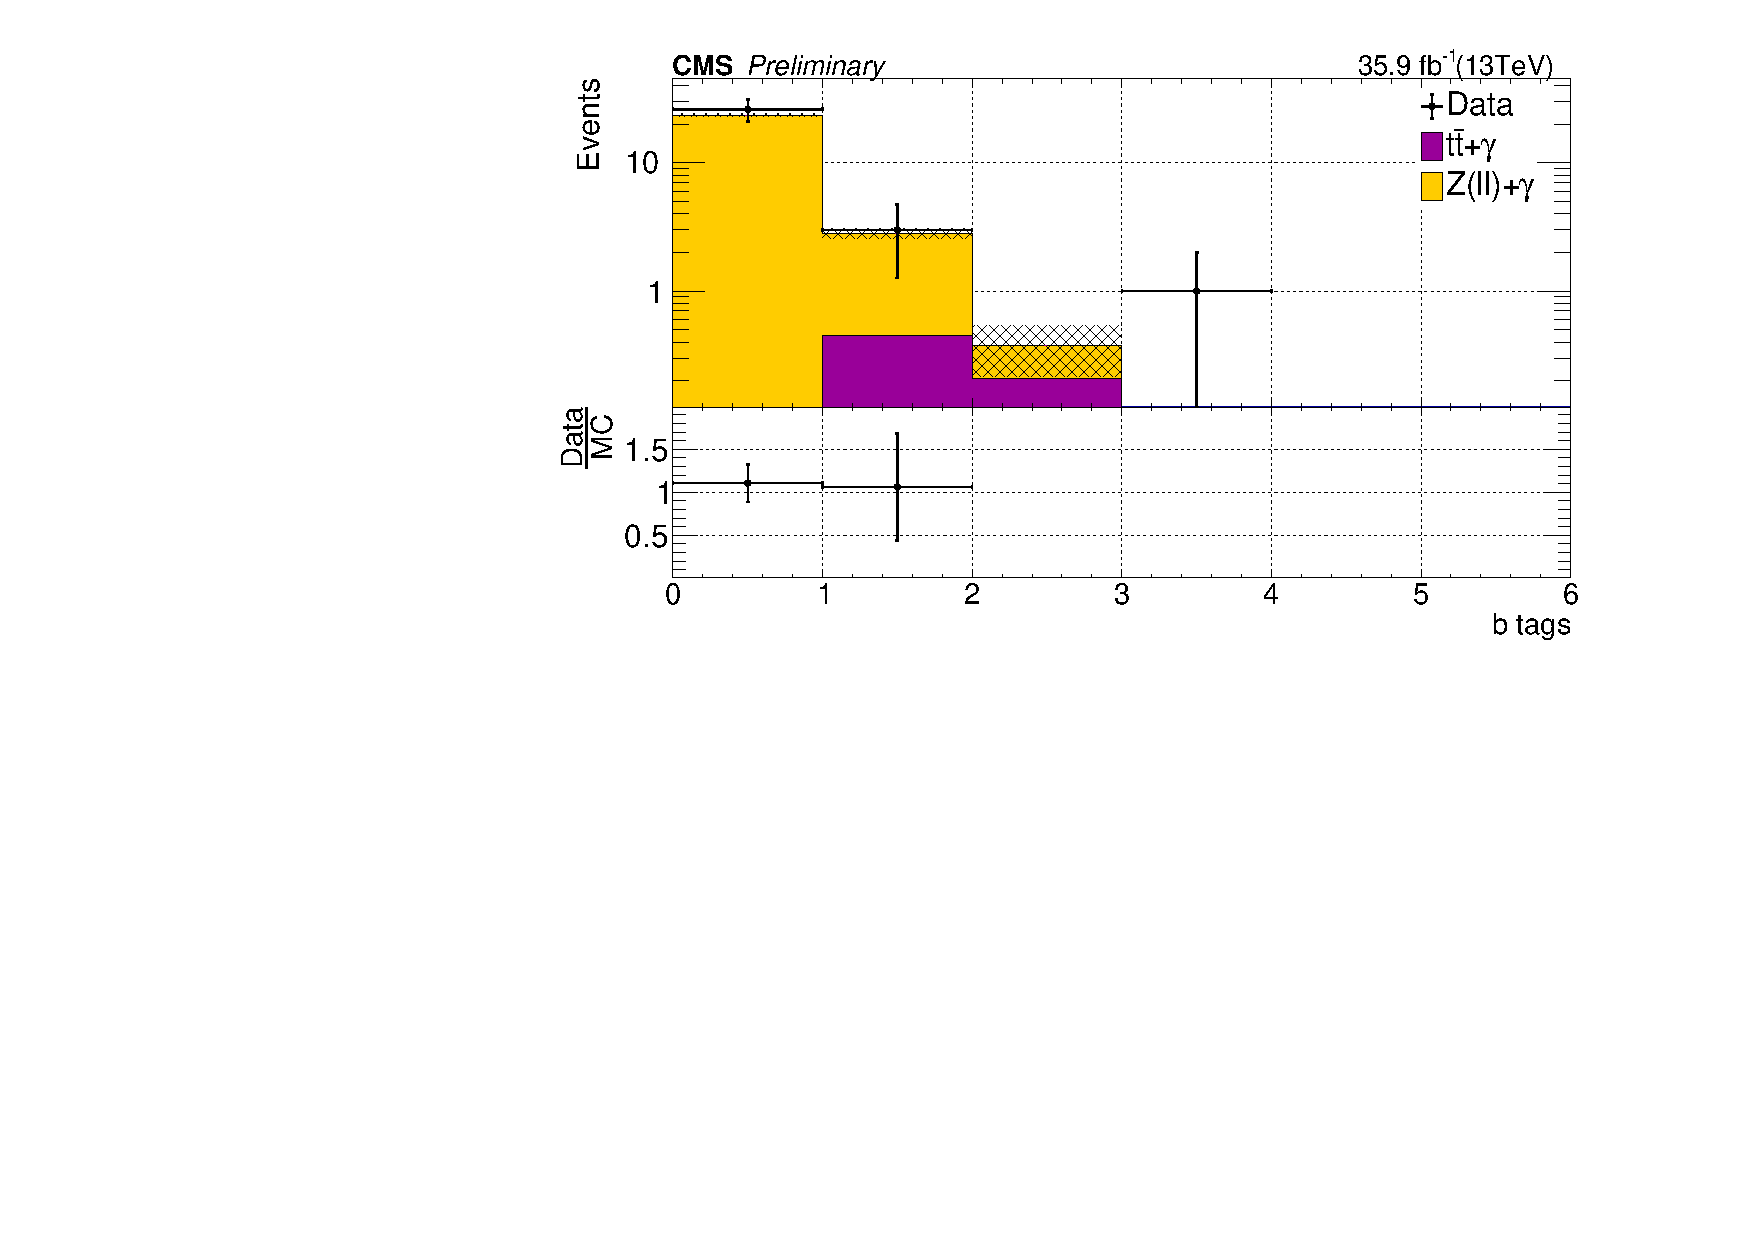
\includegraphics[width=0.48\linewidth]{../Figures/Chap3/zgamma/nBTags_LLGDataMC.pdf}
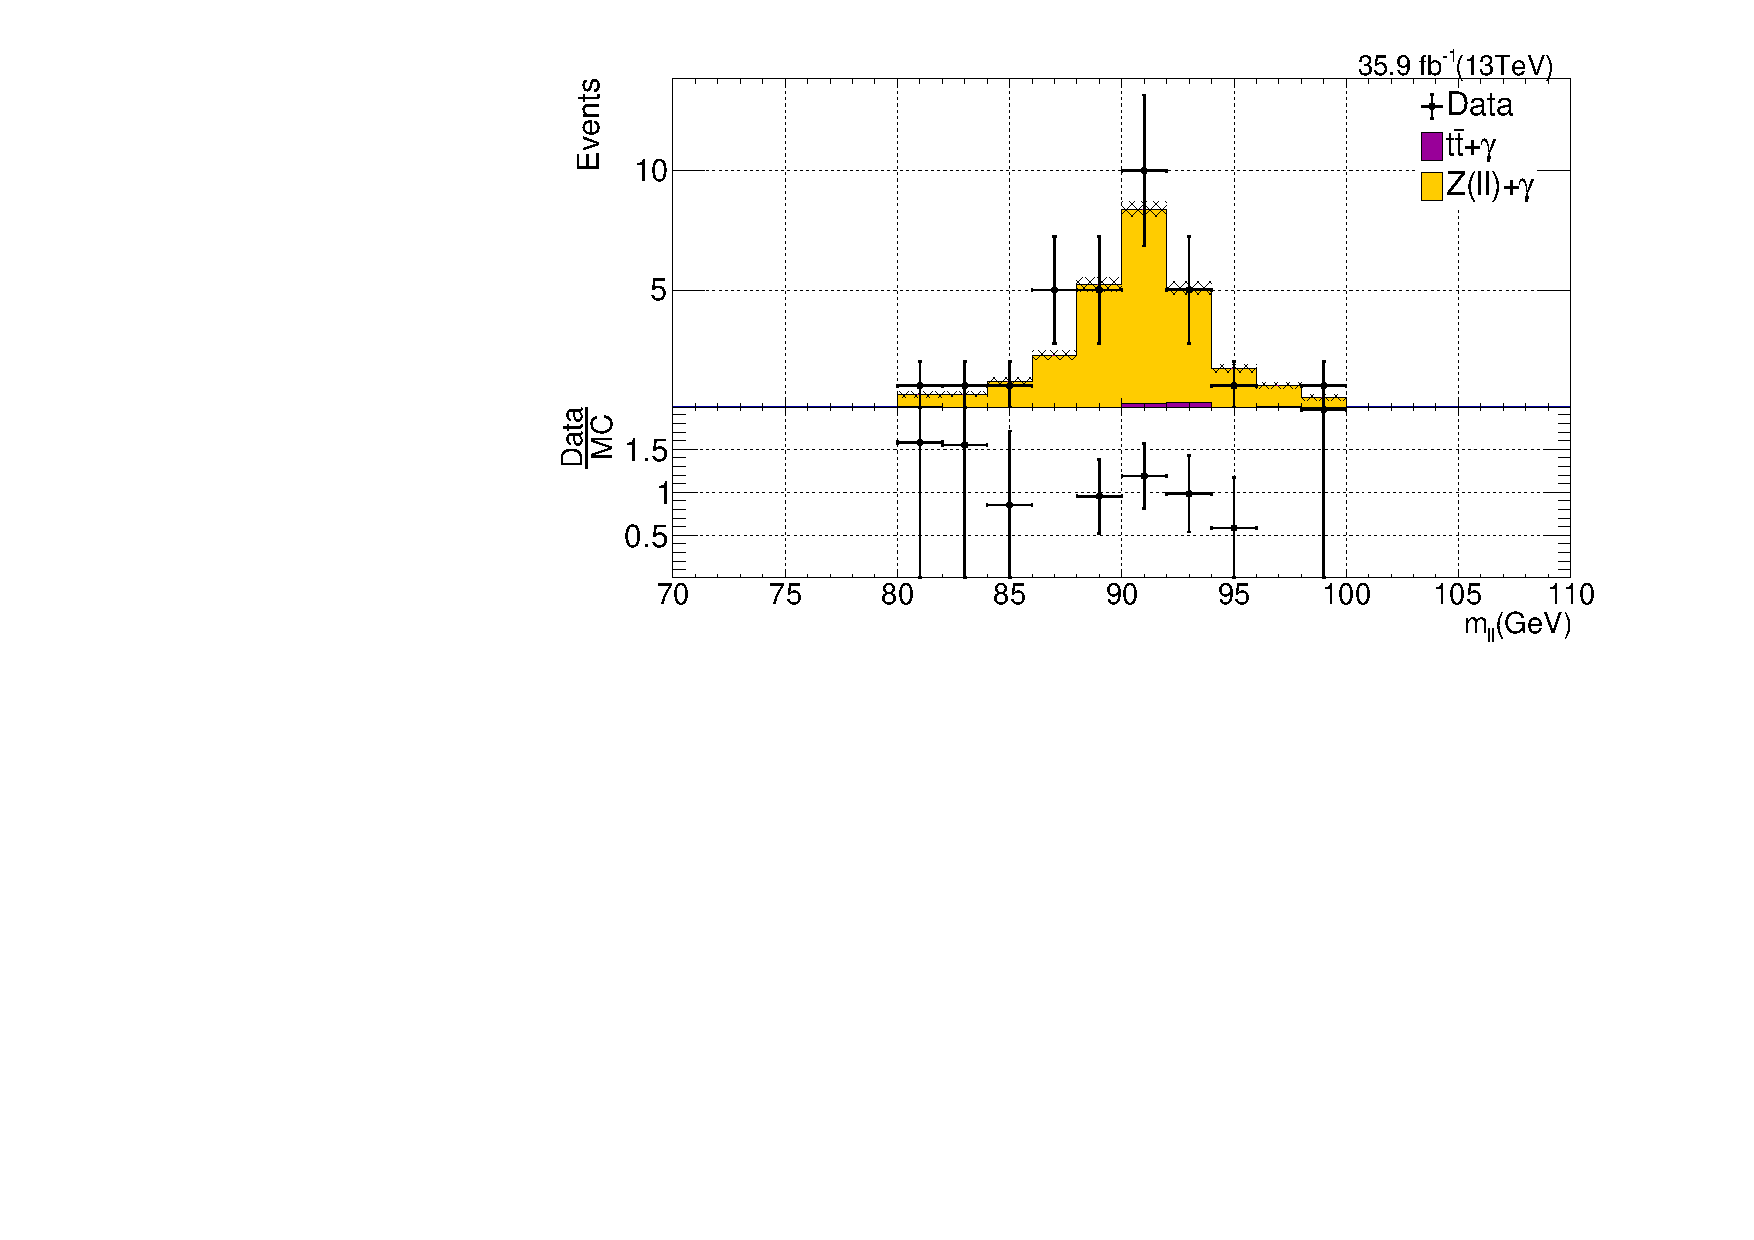
\includegraphics[width=0.48\linewidth]{../Figures/Chap3/zgamma/ZMass_LLGDataMC.pdf}
\caption[$ll+\gamma$ in data vs $ll+\gamma$ in MC]{Comparison of $ll+\gamma$ in data with $ll+\gamma$ events in MC as function of \ptmiss (top left), \nj (top right), \nb (bottom left) and $m_{\ell\ell}$ (bottom right) for $p_T^{\gamma}>190\gev$. Note that \ptmiss is calculated by ignoring the di-lepton pair. For the top left plot of \ptmiss, hashed error bars refer to statistical and EW correction uncertainties listed in Table \ref{tab:EWcorr}. For the remaining 3 plots, error bars are statistical only.}
\label{fig:llGammaDataMC}
\end{figure}

\section{Signal acceptance $\times$ efficiency}
\label{sec:SigAccEff}
Signal acceptance $\times$ efficiency is studied for different signal models and they are shown in figure \ref{fig:sigEff}. To some extent acceptance $\times$ efficiency is related to sensitivity of the analysis. Other factors such as background composition in different search bins, signal kinematics and cross section also affect the sensitivity and hence the exclusion limits. These plots are useful to in understanding some of the features seen in exclusion curves- low sensitivity near diagonal and kink for very low NLSP masses etc.
\begin{figure}[h!]
\centering
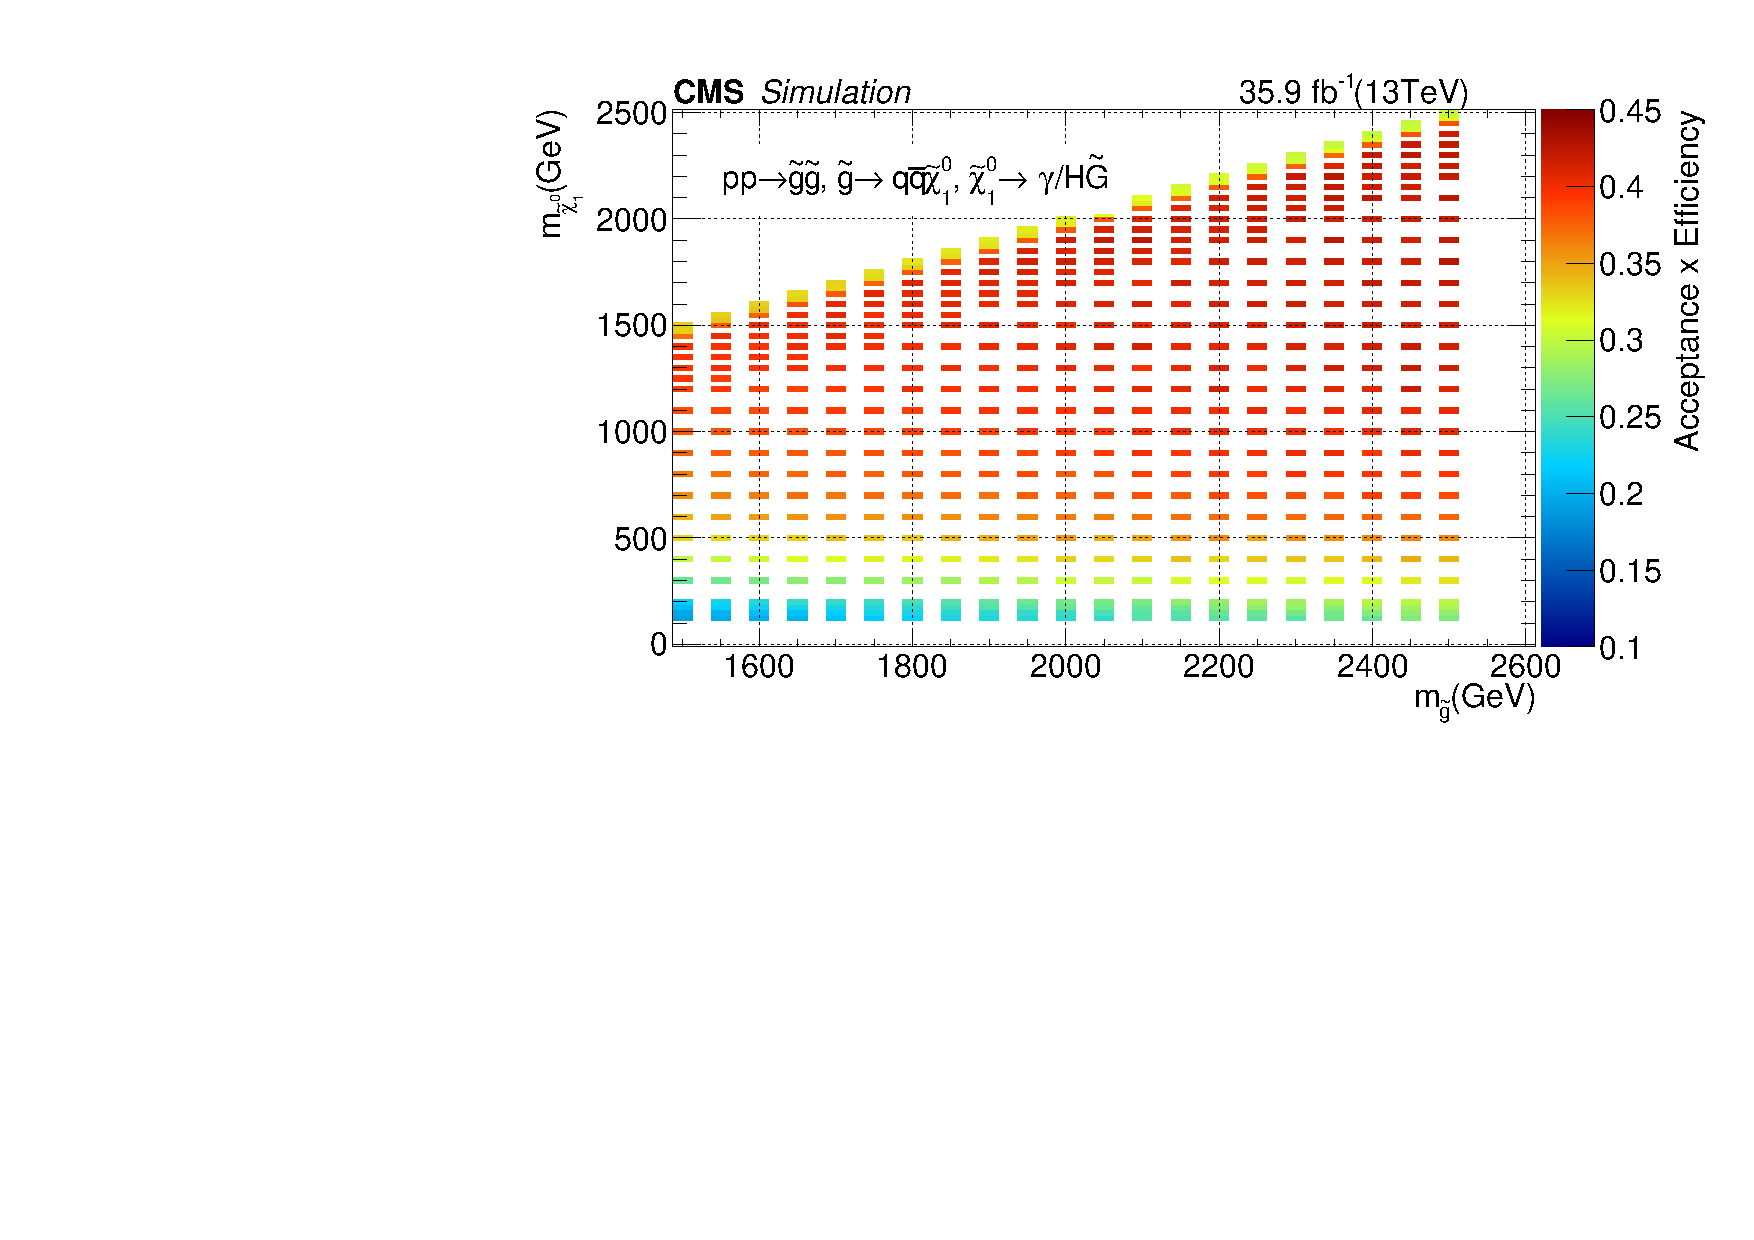
\includegraphics[width=0.46\linewidth]{../Figures/Chap3/optimization/T5qqqqHg_AccEff.pdf} \xspace
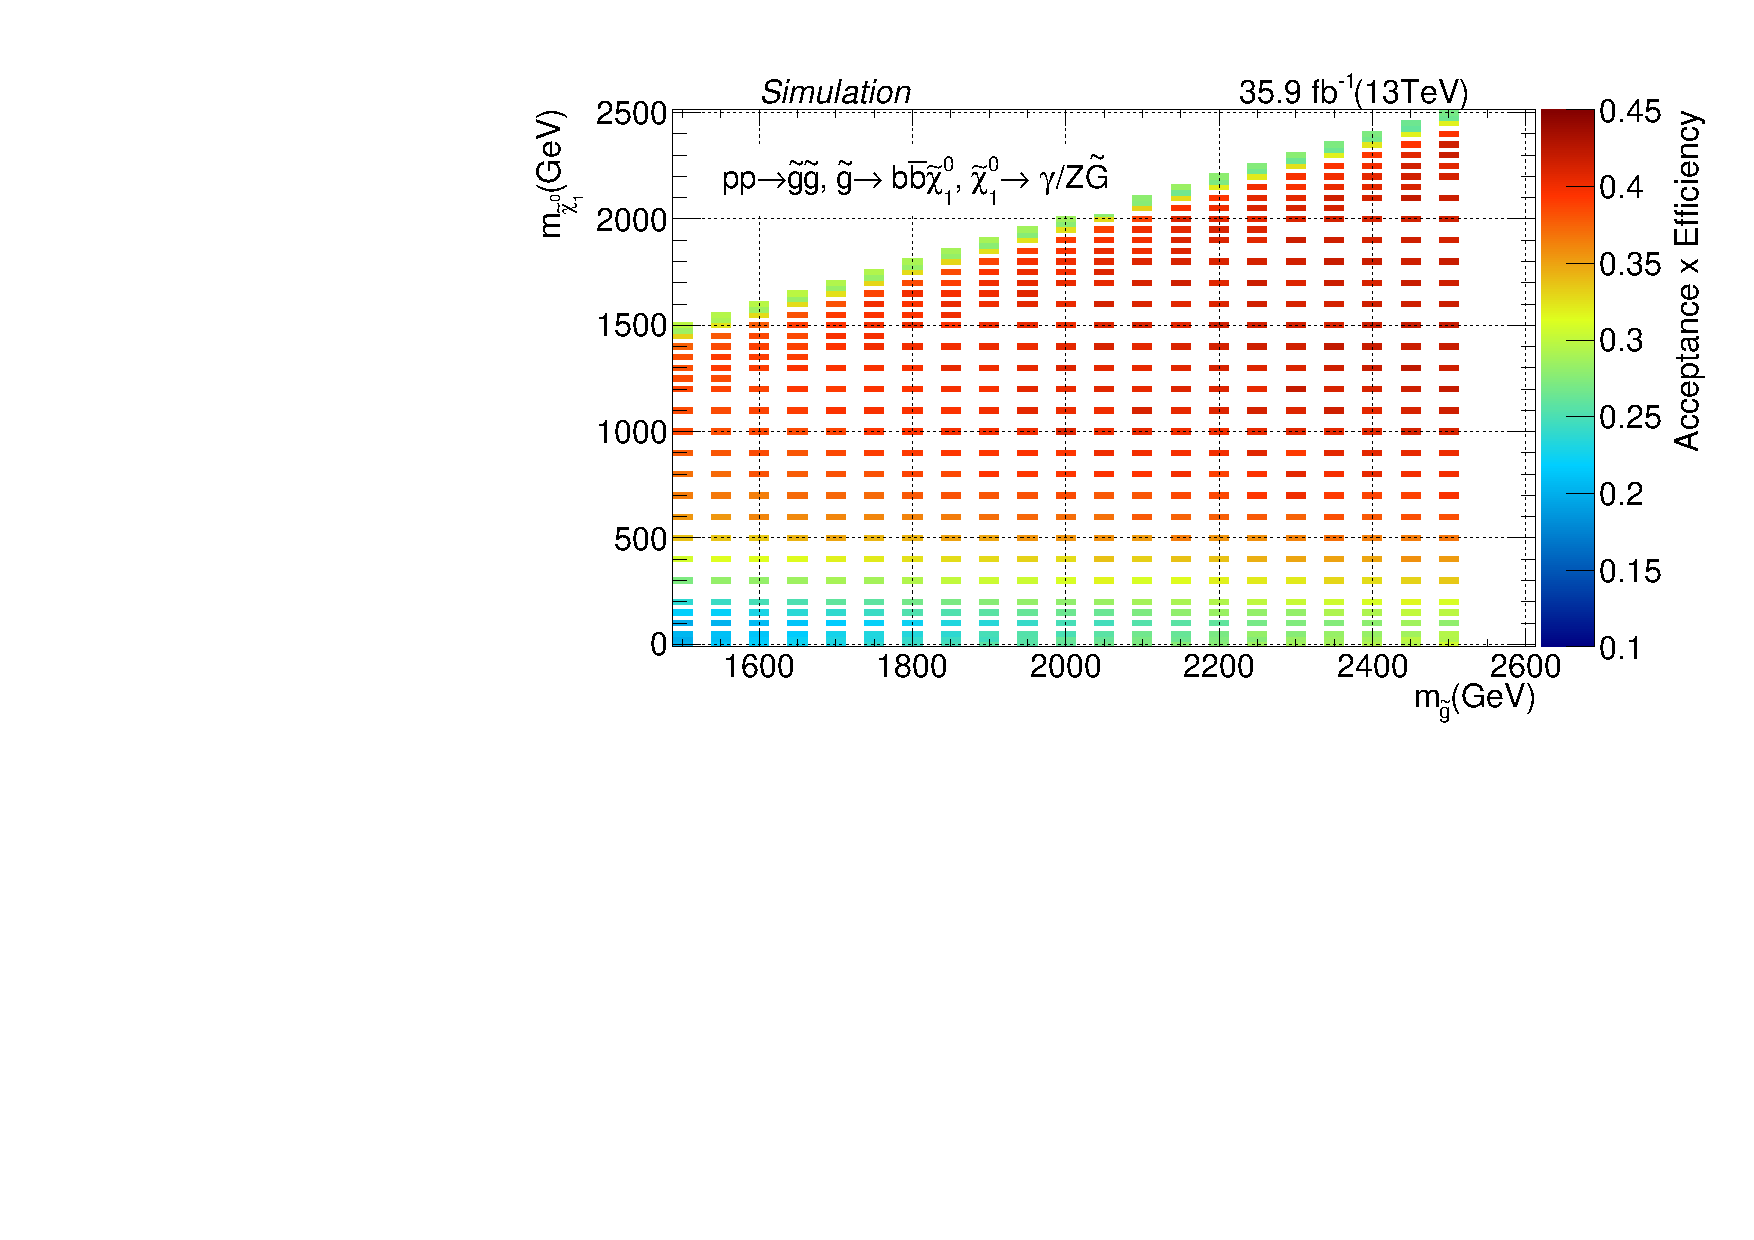
\includegraphics[width=0.46\linewidth]{../Figures/Chap3/optimization/T5bbbbZg_AccEff.pdf}\\
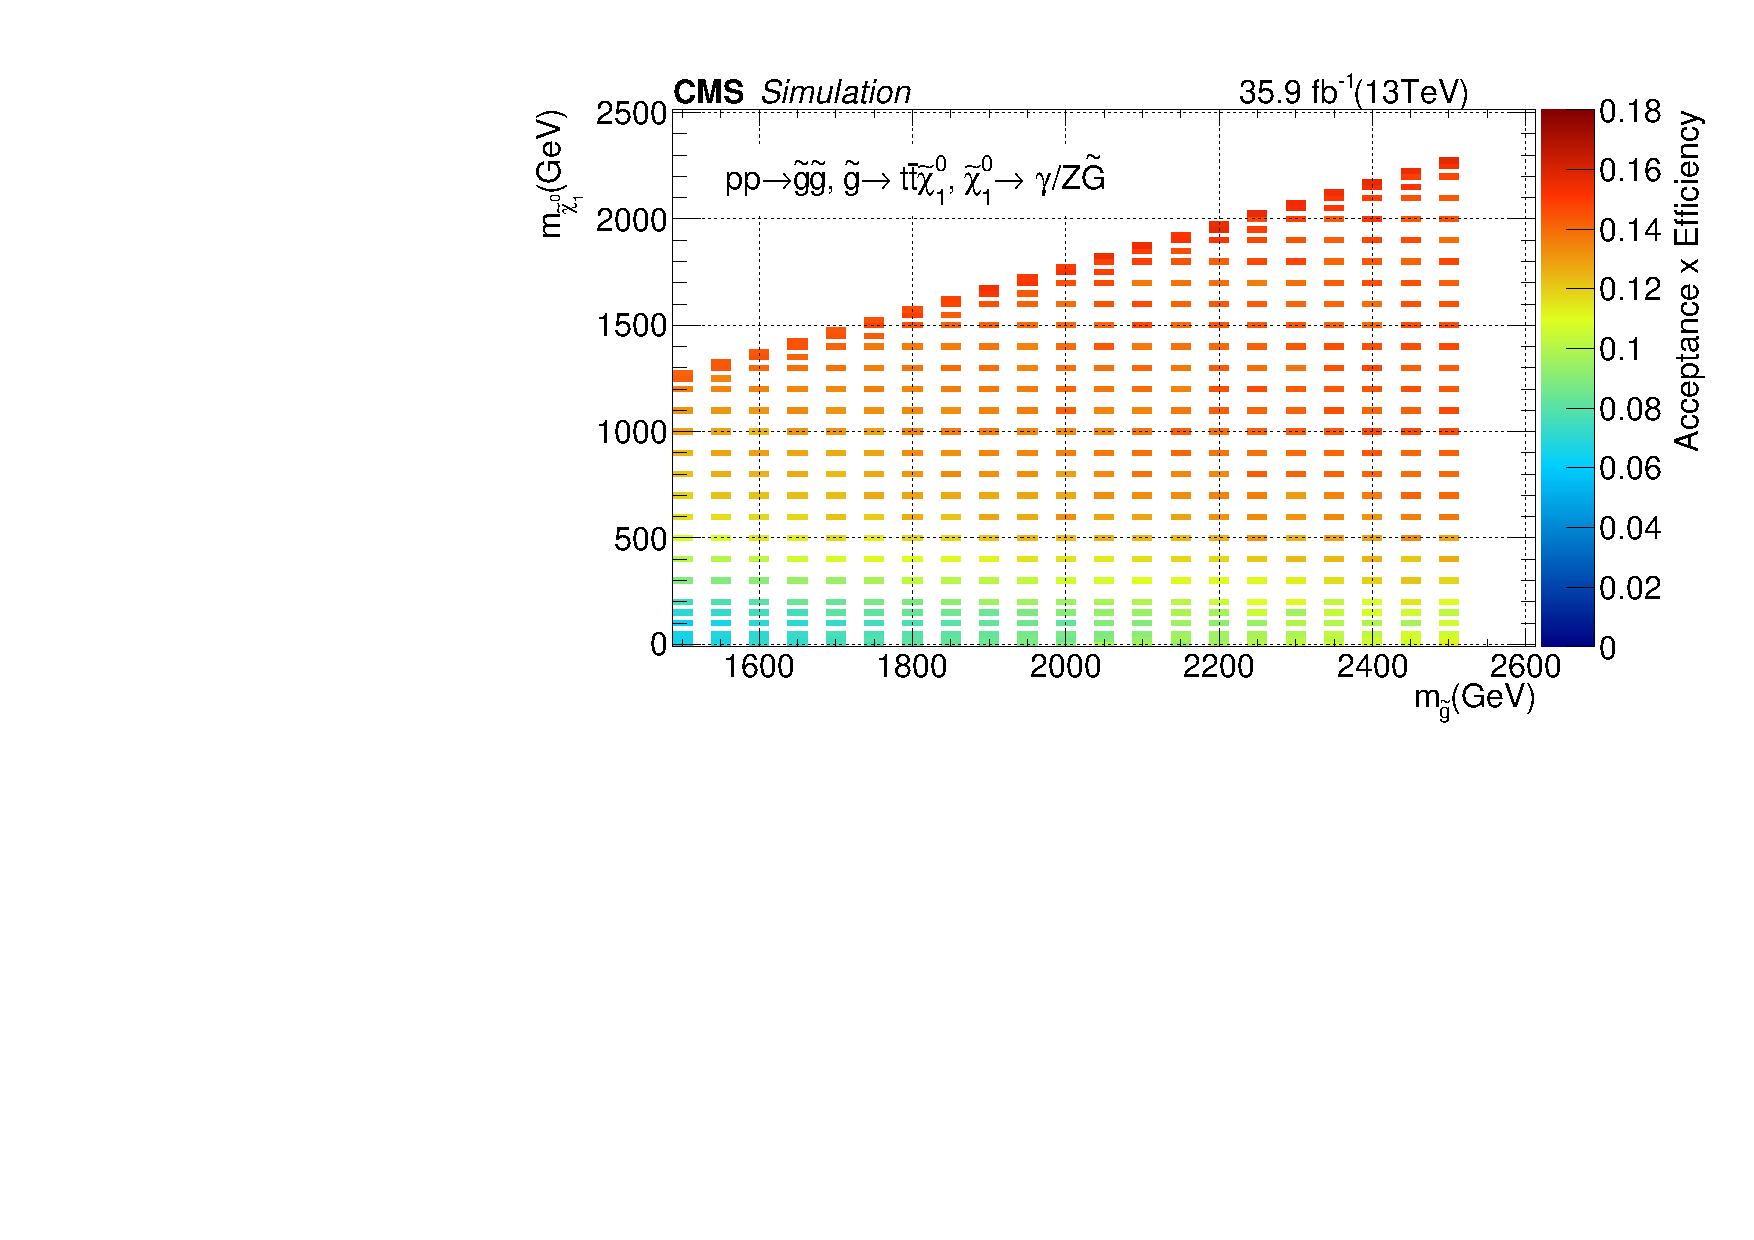
\includegraphics[width=0.46\linewidth]{../Figures/Chap3/optimization/T5ttttZg_AccEff.pdf} \xspace
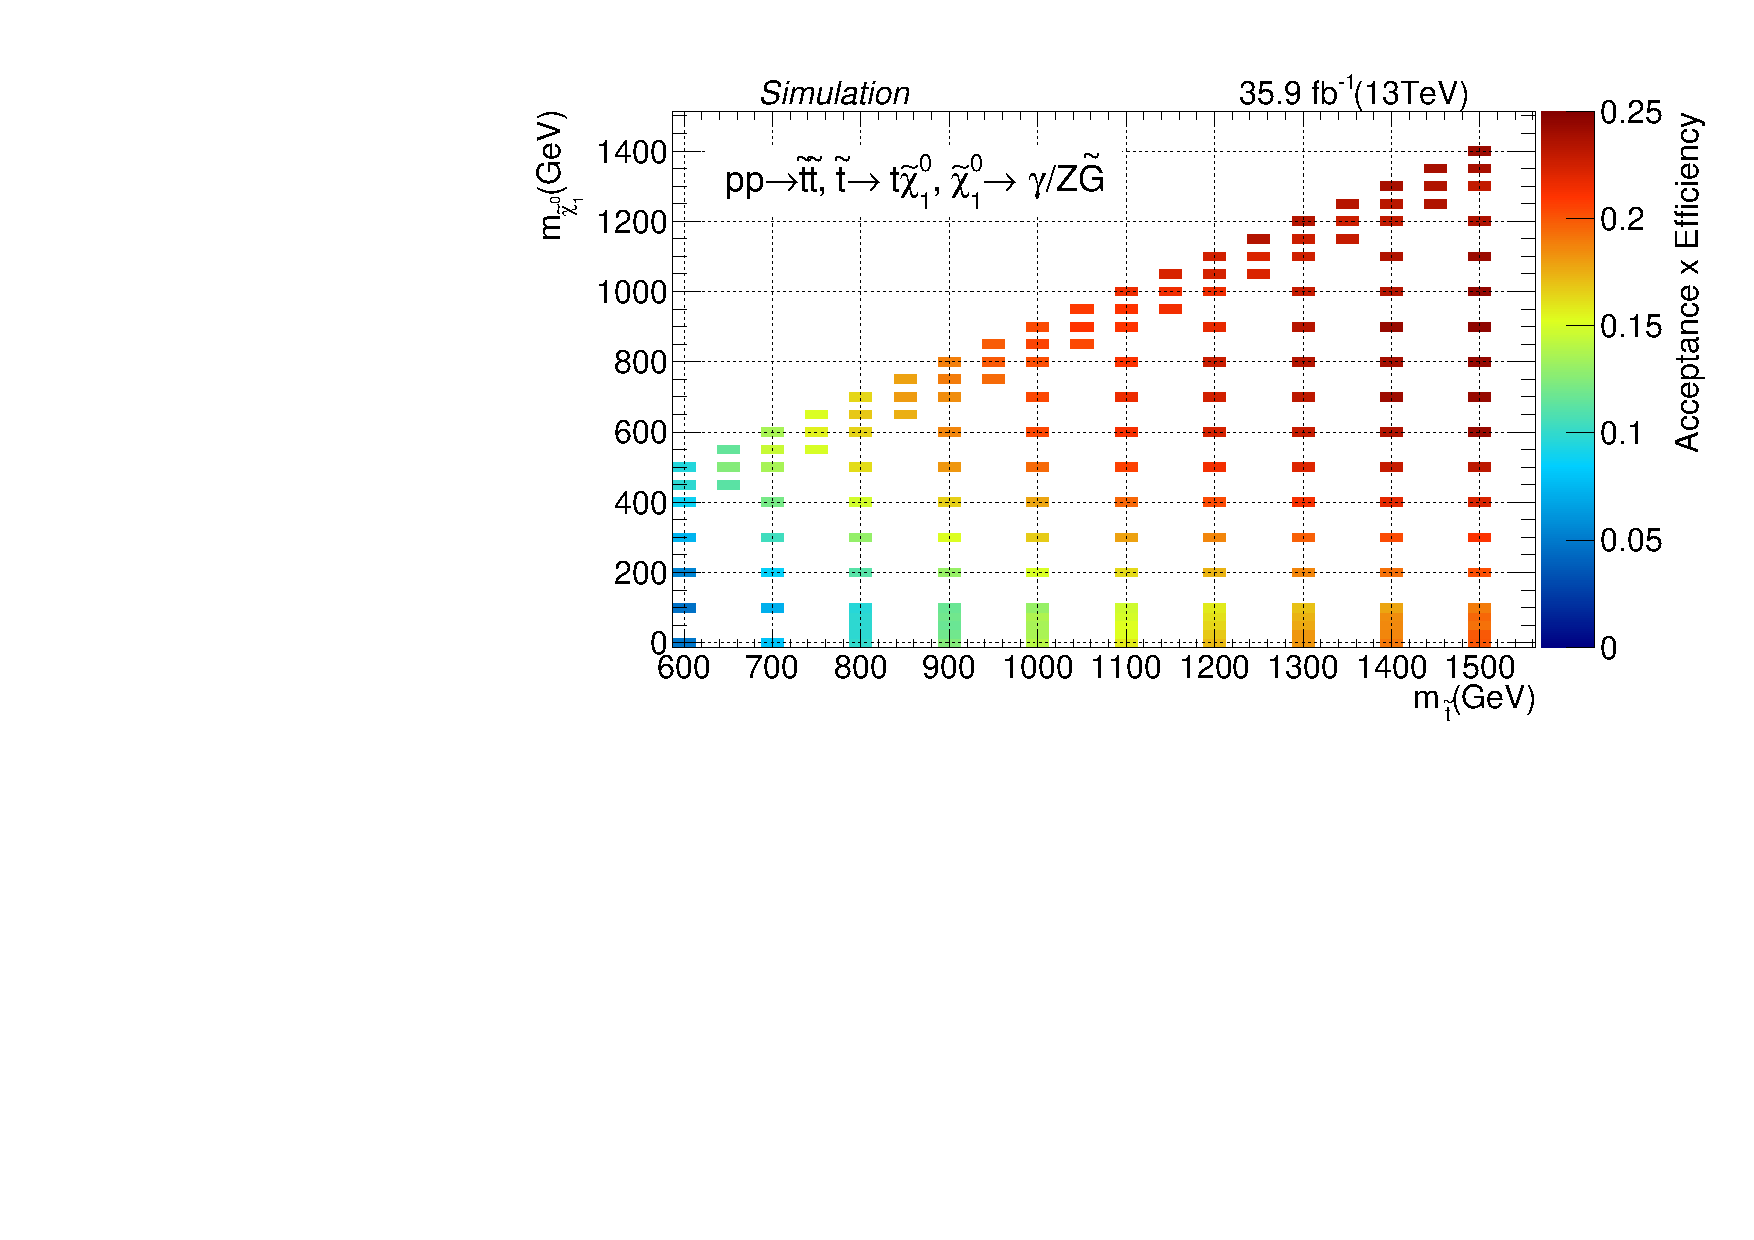
\includegraphics[width=0.46\linewidth]{../Figures/Chap3/optimization/T6ttZg_AccEff.pdf}
\caption[Acceptance $\times$ efficiency for signal]{Acceptance $\times$ efficiency for different mass points corresponding to T5qqqqHG (top left), T5bbbbZG (top right), T5ttttZG (bottom left) and T6ttZG (bottom right).}
\label{fig:sigEff}
\end{figure}